\documentclass{article} %llncs
\usepackage[T1]{fontenc}
\usepackage[utf8]{inputenc}

\usepackage[framemethod=tikz]{mdframed}
\mdfsetup{
skipabove=\baselineskip,
skipbelow=0\baselineskip,
innertopmargin=3pt,
innerbottommargin=3pt
}

%% \usepackage{fontspec}
%% \newfontfamily{\tam}[Script=Tamil]{Lohit Tamil}
%% \defaultfontfeatures{Scale=MatchLowercase}

\usepackage{eurosym}
\usepackage{hyperref}		% clickable references
\usepackage{url}
\usepackage{apacite}            % APA style citations

\usepackage{amsmath,amssymb}	% math structures and symbols
\usepackage{graphicx}		% including of graphics files in various formats
\usepackage{amsfonts}
\usepackage{dialogue}
\usepackage{placeins}
\usepackage{tikz}
\usetikzlibrary{positioning,backgrounds,fit,arrows,shapes,shadows}
\usetikzlibrary{shapes.multipart}
\usepackage{wrapfig}
\usepackage{enumitem}
\usepackage{framed}

% \hypersetup{hidelinks}

\usepackage[xspace,mla]{ellipsis}

\definecolor{myyellow}{RGB}{242,226,149}
\definecolor{mygreen}{RGB}{144,238,144}
\definecolor{mypink}{RGB}{255,182,193}
\definecolor{myorange}{RGB}{255,165,0}
\definecolor{myblue}{RGB}{0,204,204}

\usepackage{xparse}
\NewDocumentCommand\StickyNote{O{4cm}mmO{4cm}}{%
\begin{tikzpicture}
\node[
drop shadow={
  shadow xshift=2pt,
  shadow yshift=-4pt
},
inner xsep=7pt,
fill=#2,
xslant=-0.05,
yslant=0.05,
inner ysep=10pt
] {\parbox[t][#1][c]{#4}{#3}};
\end{tikzpicture}%
}

%\urldef{\mailsa}\path|{j.corneli,s.colton}@gold.ac.uk|
%\urldef{\mailsb}\path|a.pease@dundee.co.uk|

\newcommand{\keywords}[1]{\par\addvspace\baselineskip
\noindent\keywordname\enspace\ignorespaces#1}

\newcommand{\inlineitem}[1]{%
\begingroup%
\setlength\itemindent{-1em}%
\item[]%
\begin{minipage}{.96\textwidth}%
#1%
\end{minipage}%
\endgroup
}

\begin{document}

% TITLE INFORMATION
%% \title{Modelling serendipity in a computational context}
%% \author{Joseph Corneli\inst{1}, Alison Pease\inst{2}, Simon Colton\inst{1},\\ Anna Jordanous\inst{3}, Christian Guckelsberger\inst{1}}
%% \date{\today}
%% \institute{Department of Computing, Goldsmiths College, University of London\\
%% %% \mailsa\\
%% %% \mailsb\\
%% % \url{http://ccg.doc.gold.ac.uk/}
%% \and
%% School of Computing, University of Dundee
%% \and
%% School of Computing, University of Kent}

%% \maketitle

\begin{abstract}
%
Most prior work that deals with serendipity in a computing context only considers the role it plays in ``discovery'', but we argue that serendipity also includes an important ``invention'' aspect.
% \section{Literature review} \label{sec:literature-review}

In this section, we give a short overview covering the etymology of
the term ``serendipity'' and trace its development in order to pin
down the key commonalities from many definitions and instances.  In
particular, we point out key conditions of serendipity, their
components and general characteristics, including environmental
factors.  The structure of this section follows and updates an earlier
survey from \citeA{pease2013discussion}, drawing connections with our
formal model described above.

\subsection{Etymology and selected definitions} \label{sec:overview-serendipity}
The English term ``serendipity'' derives from the 1302 long poem \emph{Eight Paradises}, written in Persian by the Sufi poet Am\={\i}r Khusrow in Uttar Pradesh.\footnote{\url{http://en.wikipedia.org/wiki/Hasht-Bihisht}}  In the English-speaking world, its first chapter became known as ``The Three Princes of Serendip'', where ``Serendip'' represents the Old Tamil-Malayalam word for Sri Lanka (%{\tam சேரன்தீவு},
\emph{Cerantivu}), ``island of the Ceran kings.''

The term ``serendipity'' is first found in a 1757 letter by Horace Walpole to Horace Mann:
\begin{quote}
\emph{``This discovery is almost of that kind which I call serendipity, a very expressive
word} \ldots \emph{You will understand it better by the derivation than by the
definition. I once read a silly fairy tale, called The Three Princes of Serendip:
as their Highness travelled, they were always making discoveries, by accidents
\& sagacity, of things which they were not in quest of}[.]''~\cite[p. 633]{van1994anatomy}
\end{quote}
The term became more widely known in the 1940s through studies of serendipity as a factor in scientific discovery, surveyed by Robert Merton and Elinor Barben \citeyear{merton} in their 1957 analyis ``The Travels and Adventures of Serendipity, A Study in Historical Semantics and the Sociology of Sciences''.  Merton and Barben define the term as follows:
\begin{quote}
\emph{``The serendipity pattern refers to the fairly common experience of observing
an unanticipated, anomalous and strategic datum which becomes the occasion
for developing a new theory or for extending an existing theory.''} \cite[p. 635]{van1994anatomy}
\end{quote}
In 1986, Philippe Qu\'eau described serendipity as ``the art of
finding what we are not looking for by looking for what we are not
finding'' \cite{eloge-de-la-simulation}, as quoted in
\cite[p. 121]{Campos2002}.  Pek van Andel
\citeyear[p. 631]{van1994anatomy} describes it simply as ``the art of
making an unsought finding''.


Roberts \citeyear[pp. 246--249]{roberts} records 30 entries for the term ``serendipity'' from English language dictionaries dating from 1909 to 1989.  
%
Classic definitions require the investigator not to be aware of the problem they serendipitously solve, but this criterion has largely dropped from dictionary definitions. Only 5 of Roberts' collected definitions explicitly say ``not sought for.''  Roberts characterises ``sought findings'' in which an accident leads to a discovery with the term \emph{pseudoserendipity} \cite{chumaceiro1995serendipity}.
%
While Walpole initially described serendipity as an event, it has
since been reconceptualised as a psychological attribute, a matter of
sagacity on the part of the discoverer: a ``gift'' or ``faculty'' more
than a ``state of mind.''  Only one of the collected definitions, from
1952, defined it solely as an event, while five define it as both
event and attribute.

However, there are numerous examples that exhibit features of
serendipity which develop on a social scale rather than an individual
scale.  For instance, between Spencer Silver's creation of high-tack,
low-adhesion glue in 1968, the invention of a sticky bookmark in 1973,
and the eventual launch of the distinctive canary yellow re-stickable
notes in 1980, there were many opportunities for
Post-its\texttrademark\ \emph{not} to have come to be
\cite{tce-postits}. Accordingly, Merton and Barber argue that the
psychological perspective needs to be integrated with a
\emph{sociological} one.\footnote{ ``For if chance favours prepared
  minds, it particularly favours those at work in microenvironments
  that make for unanticipated sociocognitive interactions between
  those prepared minds. These may be described as serendipitous
  sociocognitive microenvironments'' \cite[p. 259--260]{merton}.}
Large-scale scientific and technical projects generally rely on the
``convergence of interests of several key actors''
\cite{companions-in-geography}, along with other supporting cultural
factors.  Umberto Eco \citeyear{eco2013serendipities} focuses on the
historical role of serendipitous mistakes and falsehoods in the
production of knowledge.

It is important to note that serendipity is usually discussed within
the context of \emph{discovery}, rather than \emph{creativity},
although in typical parlance these terms are closely related
\cite{jordanous12jims}.  In our definition of serendipity, we have
made use of Henri Bergson's distinction:
\begin{quote}
``\emph{Discovery, or uncovering, has to do with what already exists,
    actually or virtually; it was therefore certain to happen sooner
    or later.  Invention gives being to what did not exist; it might
    never have happened.}''~\cite{bergson2010creative}
\end{quote}
As we have indicated serendipity would seem to require features of
both; that is, the discovery of something unexpected and the invention
of an application for the same.  We must complement \emph{analysis}
with \emph{synthesis} \cite{delanda1993virtual}.  The balance between
these two features will differ from case to case.

In the next subsection we will review several historical examples.
First, one further point should be made with reference to the ``The
Three Princes of Serendip''.  Prior to Walpole's coinage, this story
had been adapted by Voltaire into an early chapter of \emph{Zadig},
and in turn ``the method of Zadig'' informed subsequent approaches
both to fiction writing and natural science.  This method is rooted
firstly in discovery:

\begin{quote}
``[Zadig] \emph{pry’d into the Nature and Properties of Animals and
    Plants, and soon, by his strict and repeated Enquiries, he was
    capable of discerning a Thousand Variations in visible Objects,
    that others, less curious, imagin’d were all
    alike.}''~\cite[pp. 21--22]{zadig}
\end{quote}

\noindent Secondly, from disparate observations, Zadig is often able
to assemble a coherent picture:
\begin{quote}
\emph{It was his peculiar Talent to render Truth as obvious as
  possible: Whereas most Men study to render it intricate and
  obscure.}~\cite[p. 54]{zadig}
\end{quote}
Similarly, but in reverse, a coherent picture may be reduced to
fragmented pieces each of which may tell a very different story from
the whole.  This is illustrated in Zadig's misadventure with a broken
tablet, in which one fragment of a poem of praise reads as treasonous
provocation.  In describing the various features of serendipity below,
we will draw connections with the schematic diagram presented in
Section \ref{specs-overview}, in order to unfold the multifaceted
notion of serendipity.

\subsection{Connections between prior literature on serendipity and our formal definition} \label{sec:connections-to-formal-definition}

\subsubsection*{Key condition for serendipity}

\begin{itemize}
\item \textbf{Focus shift}: ``\emph{After removing several of the
  burdock burrs (seeds) that kept sticking to his clothes and his
  dog's fur,}~[de Mestral]~\emph{became curious as to how it
  worked. He examined them under a microscope, and noted hundreds of
  `hooks' that caught on anything with a loop, such as clothing,
  animal fur, or hair. He saw the possibility of binding two materials
  reversibly in a simple fashion, if he could figure out how to
  duplicate the hooks and loops.}''~\cite{wiki:velcro}
%
\inlineitem{This corresponds to the identification of $T^\star$, which
  is common to both sides of the diagram.  \citeA{creativity-crisis}
  write that: ``To be creative requires divergent thinking (generating
  many unique ideas) and then convergent thinking (combining those
  ideas into the best result).''  Accordingly $T^\star$ may be thought
  of as an evolving vector of interesting possibilities or ``strategic data'' \cite[p. 507]{merton1948bearing}.  In de
  Mestral's case, the initial idea of a hook-and-loop fastener
  occurred in 1941 -- followed by a full decade of experimentation
  before he was ready to file a patent claim.  }
\end{itemize}

\subsubsection*{Components of serendipity}

\begin{itemize}
\item \textbf{Prepared mind}: 
Fleming's ``prepared mind'' included his focus
on carrying out experiments to investigate influenza as well as his
previous experience that foreign substances in petri dishes can kill
bacteria.  He was concerned above all with the question ``Is there a
substance which is harmful to harmful bacteria but harmless to human
tissue?''  \cite[p. 161]{roberts}.
%%
%
\inlineitem{This corresponds to the prior
  training $p$ and $p^{\prime}$ in our diagram.}
\item \textbf{Serendipity trigger}: The trigger does not directly
  cause the outcome, but rather, inspires a new insight.  It was long
  known by Quechua medics that cinchona bark stops shivering.  In
  particular, it worked well to stop shivering in malaria patients, as
  was observed when malarial Europeans first arrived in Peru.  The
  joint appearance of shivering Europeans and a South American remedy
  was the trigger.  That an extract from cinchona bark can cure and
  can even prevent malaria was subsequently revealed.
%
\inlineitem{This corresponds to the stimulus $T$ in our diagram.}
%%
\item \textbf{Bridge}: These include reasoning techniques, such as
  abductive inference (what might cause a clear patch in a petri
  dish?); analogical reasoning (de Mestral constructed a target domain
  from the source domain of burs hooked onto fabric); and conceptual
  blending (Kekul\'e blended his knowledge of molecule structure with
  his vision of a snake biting its tail).  The bridge may also rely on
  new social arrangements, such as the formation of cross-cultural
  research networks.
%
\inlineitem{This corresponds to the actions based on $p^{\prime}$
  taken on $T^\star$ leading to $R$.}
%%
\item \textbf{Result}: This may be a new product, artefact, process,
  hypothesis, a new use for a material substance, and so on.  The
  outcome may contribute evidence in support of a known hypothesis, or
  a solution to a known problem.  Alternatively, the result may itself
  be a {\em new} hypothesis or problem.  The result may be a
  ``pseudoserendipitous'' in the sense that it was {\em sought}, while
  nevertheless arising from an unknown, unlikely, coincidental or
  unexpected source.  More classically, it is an \emph{unsought}
  finding, such as the discovery of the Rosetta stone.
%
\inlineitem{This corresponds to our $R$.  Note that $R$ may imply
  updates to $p$ or $p^{\prime}$ in further phases of research.}
\end{itemize}

\subsubsection*{Dimensions of serendipity}

Whereas the foregoing items are the central features of the
definition, the following further characterise the circumstances under
which serendipity occurs in practice.

\begin{itemize}
\item \textbf{Chance}: Fleming \citeyear{fleming} noted: ``There are
  thousands of different moulds'' -- and ``that chance put the mould
  in the right spot at the right time was like winning the Irish
  sweep.''
%
\inlineitem{One must assume that relatively few triggers $T^\star$
  that are identified as interesting actually lead to useful results;
  in other words, the process is fallible.}
%%
\item \textbf{Curiosity}: Venkatesh Rao \citeyear{rao2011tempo} refers
  to a \emph{cheap trick} that takes place early on in a narrative in
  order to establish the preliminary conditions of order.  Curiosity
  with can play this role, and can dispose a creative person to begin,
  or to continue, a search into unfamiliar territory.
%
\inlineitem{The prior training $p$ causes interesting features to be
  extracted, even if they are not necessarily useful; $p^{\prime}$
  asks how these features \emph{might} be useful.  }
%%
\item \textbf{Sagacity}: This old-fashioned word is related to
  ``wisdom,'' ``insight,'' and especially to ``taste'' -- and
  describes the attributes, or skill, of the discoverer that
  contribute to forming the bridge between the trigger and the result.
  In many cases, such as an entanglement with cockle-burs, many others
  will have already been in a similar position and not obtained an
  interesting result.  Once a phenomenon has been identified as
  interesting, the disposition of the investigator may lead to a
  dogged pursuit of a useful application or improvement.
%
\inlineitem{Rather than a simple look-up
  rule, $p^{\prime}$ involves creating new knowledge.}
%%
\item \textbf{Value}: Note that the chance ``discovery'' of, say, a
  \pounds 10 note may be seen as happy by the person who finds it,
  whereas the loss of the same note would generally be regarded as
  unhappy.  Positive judgements of serendipity by a third party would
  be less likely in scenarios in which ``One man's loss is another
  man's gain'' than in scenarios where ``One man's trash is another
  man's treasure.''  If possible we prefer this sort of independent
  judgement \cite{jordanous:12}.
%
\inlineitem{The evaluation $|R|>0$ may be carried out ``locally'' (as
  an embedded part of the process of invention of $R$) or ``globally''
  (i.e.~as an external process).  }
\end{itemize}

\subsubsection*{Environmental factors}

\begin{itemize}
\item \textbf{Dynamic world}: Information about the world develops
  over time, and is not presented as a complete, consistent whole.  In
  particular, value may come later.  Van Andel
  \citeyear[p. 643]{van1994anatomy} estimates that in twenty percent
  of innovations ``something was discovered before there was a demand
  for it.''
%
\inlineitem{$T$ (and $T^\star$) appears within a stream of data with
  indeterminacy.  There is a further feedback loop, insofar as
  products $R$ influence the future state.}
%%
\item \textbf{Multiple contexts}: One of the dynamical aspects at play
  may be the discoverer going back and forth between different
  contexts, with different stimuli.  3M employee Arthur Fry sang in a
  church choir and needed a good way to mark pages in his hymn book;
  he happened to have been attending seminars offered by his colleague
  Silver about restickable glue.
%
\inlineitem{This is reflected directly in our model by the difference
  between the ``context of discovery'' involving prior preparations
  $p$, and the ``context of invention'' involving prior preparations
  $p^{\prime}$.  Both of these may be subdivided further.}
%%
\item \textbf{Multiple tasks}: Even within what would typically be
  seen as a single context, a discoverer may take on multiple tasks
  that segment the context into sub-contexts, or that cause the
  investigator to look in more than one direction.  The tasks may have
  an interesting \emph{overlap}, or they may point to a \emph{gap} in
  knowledge.  As an example of the latter, Penzias and Wilson used a
  large antenna to detect radio waves that were relayed by bouncing
  off of satellites.  After they had removed interference effects due
  to radar, radio, and heat, they found residual ambient noise that
  couldn't be eliminated \cite{wiki:cosmic-radiation}.
%
\inlineitem{Both $T$ and $T^\star$ may be multiple, causing an
  individual process to fork into communicating sub-processes that
  involve different skills sets.}
%%
\item \textbf{Multiple influences}: The ``bridge'' from trigger to
  result is often found through a social network, thus, for instance
  Penzias and Wilson only understood the significance of their work
  after reading a preprint by Jim Peebles that hypothesised the
  possibility of measuring radiation released by the big bang
  \cite{wiki:cosmic-radiation}.
%
\inlineitem{The process as a whole may be multiplied out among
  different communicating investigators.}
\end{itemize}

We survey literature describing serendipitous discovery+invention in science and technology.
% \section{Serendipity in a computational context} \label{sec:computational-serendipity}

The 13 criteria from Section \ref{sec:literature-review}
specify the conditions and preconditions that are conducive to
serendipitous discovery.  Here, we revisit each of these criteria and
briefly summarise how they can be thought about from a computational
point of view.
% What is the goal of the computation (input and output)
% Why is it appropriate (formal spec e.g. considering externalities)
% what is the logic of the strategy by which it can be carried out.

\textbf{[Do we need to include the partial repetition below or is the
    above formal enough?  Could these bulleted ideas be condensed into
    one or two paragraphs]}

\subsubsection*{Key condition for serendipity}

\begin{itemize}
\item \textbf{Focus shift}: A focus shift is linked to re-evaluation
  of data, processes, or products.  It may precipitate changes in the
  entire framework of evaluation or its effects may be more contained.
  Such reevaluation could be modelled using a multi-agent
  architecture, in which each agent has a goal and evaluates generated
  products relative this goal, but in which agents also share their
  products with other, who then evaluate them against their own
  metrics.
\end{itemize}

\subsubsection*{Components of serendipity}

\begin{itemize}
\item \textbf{Prepared mind}: This comprises the background knowledge,
  unsolved problems, current goal, programming, and operating
  environment of a computational system.
%%
\item \textbf{Serendipity trigger}: The generation or observation of a
  potentially novel example, concept, or conjecture, etc., which
  precedes a discovery in a computational system.\footnote{Triggers
    are often examples without an explanation, rather than
    wholly-formed concepts.}  The trigger is outside of the direct
  control of the system components responsible for evaluations.
%%
\item \textbf{Bridge}: Reasoning and/or programmatic interaction
  brings about a focus shift at an opportune juncture, building on
  prior preparation and on the serendipity trigger.  The bridge may be
  constructed on the basis of logical methods, analogies, conceptual
  blending, evolutionary search, automated theory formation and may
  draw on interactions with other systems.
%%
\item \textbf{Result}: The discovery itself may be a new product,
  artefact, process, hypothesis, use for an object, etc., generated by
  computational means, which may influence the future operations of
  the system.
\end{itemize}

\subsubsection*{Dimensions of serendipity}

\begin{itemize}
\item \textbf{Chance}: Controlled randomness in AI systems is
  well-established, e.g. in Genetic Algorithms and search.  Chance
  also applies in connection with an under-determined outside world
  (see below).
%%
\item \textbf{Curiosity}: The system needs to expend discretionary
  computational effort on the serendipity trigger.  This may be
  accompanied by system features that an observer would describe as
  playfulness, inventiveness, and the drive to experiment or
  understand.
%%
\item \textbf{Sagacity}: Sagacity be modelled by employing reasoning
  over multiple application domains simultaneously; or, again, with a
  social analogue in cases where the system does not know, but ``knows
  who to ask.''
%%
\item \textbf{Value}: The result should be interesting or useful, as
  judged by the system, the programmer, the user, or another party
  (potentially another system).
\end{itemize}

\subsubsection*{Environmental factors}

\begin{itemize}
\item \textbf{Dynamic world}: Connections with other systems, data
  sources, or user input, e.g., via the web, which is highly dynamic --
  or in the context of a larger simulation.
%%
\item \textbf{Multiple contexts}: Reasoning which operates across
  domains, such as analogical reasoning, or that considers multiple
  perspectives, as in systems with social awareness.
%%
\item \textbf{Multiple tasks}: Multiple goals or targets that compete
  for resources.  The system may be implemented using a multithreaded,
  parallel processing design.
%%
\item \textbf{Multiple influences}: This may again be modelled as a
  multi-agent systems, as or multiple interacting systems, each with
  different knowledge and goals.  The source of unexpectedness may be
  arise on various levels, and a system may bring this to bear using
  techniques of reflection.
\end{itemize}

% \subsection{Proposed experiment: A Writers Workshop for Systems} \label{sec:writers-workshop}

Richard Gabriel \cite{gabriel2002writer} describes the practise of
Writers Workshops that has been put to use for over a decade within
the Pattern Languages of Programming (PLoP) community.  The basic
style of collaboration originated much earlier with groups of literary
authors who engage in peer-group critique.  Some literary workshops
are open as to genre, and happy to accommodate beginners, like the
Minneapolis Writers
Workshop\footnote{\url{http://mnwriters.org/how-the-game-works/}};
others are focused on professionals working within a specific genre,
like the Milford Writers
Workshop\footnote{\url{http://www.milfordsf.co.uk/about.htm}}.  The
practices that Gabriel describes are fairly typical.  Authors come
with work ready to present, and read a short sample, which is then
discussed and constructively critiqued by attendees.  Presenting
authors are not permitted to rebut these comments.  The commentators
generally summarise the work and say what they have gotten out of it,
discuss what worked well in the piece, and talk about how it could be
improved.  The author listens and may take notes; at the end, he or
she can then ask questions for clarification.  Generally, non-authors
are either not permitted to attend, or are asked to stay silent
through the workshop, and perhaps sit separately from the
participating authors/reviewers.  There are similarities between the
Writers Workshops and classical practices of group composition
\cite{jin1975art} and dialectic \cite{dialectique}, and the workshop
may be considered an artistic or creative space in its own right.

In PLoP workshops, authors present design patterns and pattern
languages, or papers about patterns, rather than more traditional
literary forms like poems, stories, or chapters from novels.  Papers
must be workshopped at a PLoP or EuroPLoP conference in order to be
considered for the \emph{Transactions on Pattern Languages of
  Programming} journal.  A discussion of writers workshops
in the language of design patterns is presented by
Coplien and Woolf \cite{coplien1997pattern}.  Their patterns include:
\begin{center}
{\small
\begin{tabular}{l@{\hspace{.2cm}}l@{\hspace{.2cm}}l}
\emph{Open Review} & \emph{Safe Setting} & \emph{Workshop Comprises Authors} \\
\emph{Authors are Experts} & \emph{Community of Trust} & \emph{Moderator Guides the Workshop} \\
\emph{Thank the Author} & \emph{Selective Changes} & \emph{Clearing the Palate} \\
\end{tabular}
}
\end{center}

We propose that a similar pattern-based approach should be deployed
within the Computational Creativity community to design a workshop in
which the participants are computer systems instead of human authors.
The annual International Conference on Computational Creativity
(ICCC), now entering its sixth year, could be a suitable venue.
Rather than the system's creator presenting the system in a
traditional slideshow and discussion, or a system ``Show and Tell,''
the systems would be brought to the workshop and would present their
own work to an audience of other systems, in a Writers Workshop
format.  This might be accompanied by a short paper for the conference
proceedings written by the system's designer describing the system's
current capabilities and goals.  Subsequent publications might include
traces of interactions in the Workshop, commentary from the system on
other systems, and offline reflections on what the system might change
about its own work based on the feedback it receives.  As in the PLoP
community, it could become standard to incorporate this sort of workshop
into the process of peer reviewing journal articles for the new \emph{Journal of
  Computational Creativity}\footnote{\url{http://www.journalofcomputationalcreativity.cc}}.

\begin{table}[p]
\begin{tabular}{lp{.7\textwidth}}
{\bf\emph{Successful error}} & \\
\emph{Van Andel's example}: & Post-it\texttrademark\ notes \\[.2cm]
{\tt presentation}& Systems should be prepared to share interesting ideas even if they don't know directly how they will be useful.  \\
{\tt listening}   & Systems should listen with interest, too. \\
{\tt feedback}    & Even interesting ideas may not be ``marketable.''\\
{\tt questions}   & How is your suggestion useful? \\
{\tt reflections} & New combinations of ideas take a long time to realise, and many different ideas may need to be combined in order to come up with something useful.\\
\end{tabular}
\bigskip

\begin{tabular}{lp{.7\textwidth}}
{\bf\emph{Side effect}} & \\
\emph{Van Andel's example}: & Nicotinamide used to treat side-effects of radiation therapy proves efficacious against tuberculosis. \\[.2cm]
{\tt presentation}& Systems should use their presentation as an experiment. \\
{\tt listening}   & Listeners should allow themselves to be affected by what they are hearing. \\
{\tt feedback}    & Feedback should convey the nature of the effect.\\
{\tt questions}   & The presenter may need to ask follow-up questions to gain insight. \\
{\tt reflections} & Form a new hypothesis before seeking a new audience. \\
\end{tabular}
\bigskip

\begin{tabular}{lp{.7\textwidth}}
{\bf\emph{Wrong hypothesis}} & \\
\emph{Van Andel's example}: & Lithium, used in a control study, had an unexpected calming effect. \\[.2cm]
{\tt presentation}& How is this presentation interpretable as a (``natural'') control study? \\
{\tt listening}   & Listeners are ``guinea pigs''.\\
{\tt feedback}    & Discuss side-effects that do not necessarily correspond to the author's perceived intent. \\
{\tt questions}   & Zero in on the most interesting part of the conversation.\\
{\tt reflections} & Revise hypotheses to correspond to the most surprising feedback. \\
\end{tabular}
\bigskip

\begin{tabular}{lp{.7\textwidth}}
{\bf\emph{Outsider}} & \\
\emph{Van Andel's example}: & A mother suggests a new hypothesis to a doctor. \\[.2cm]
{\tt presentation}& The presenter is here to learn from the audience. \\
{\tt listening}   & The audience is here to give help, but also to get help.\\
{\tt feedback}    & Feedback will inevitably draw on previous experiences and ideas.\\
{\tt questions}   & What is the basis for that remark?\\
{\tt reflections} & How can I implement the suggestions?\\
\end{tabular}
\vspace{.2cm}
\caption{Reinterpreting patterns of serendipity for use in a computational workshop\label{tab:reinterpret}}
\end{table}

\begin{figure}[t]
\begin{center}
\resizebox{.93\textwidth}{!}{
\StickyNote[2.5cm]{myyellow}{{\LARGE {Interesting idea}} \\[4ex] {Surprise birthday party}}[3.8cm] \StickyNote[2.5cm]{mygreen}{{\Large I heard you say:} \\[4ex] {``surprise''} }[3.8cm]
\StickyNote[2.5cm]{pink}{{\Large Feedback:} \\[4ex] {I don't like surprises}}[3.8cm]
}
\resizebox{.61\textwidth}{!}{
\StickyNote[2.5cm]{myorange}{{\LARGE {Question}} \\[4ex] {Not even a little bit?\ldots}}[3.8cm]
\quad \raisebox{-.2cm}{\StickyNote[2.5cm]{myblue}{{\LARGE Note to self:} \\[4ex] {(Try smaller surprises \\ next time.)}}[3.8cm]}
}
\end{center}
\caption{A paper prototype for applying the \emph{Successful Error} pattern\label{fig:paper-prototype}}
\end{figure}

In order to facilitate this sort of interaction, it would be necessary
for systems to implement a basic protocol related to
%%
\[
\text{
{\tt presentation}, {\tt listening}, {\tt
  feedback}, {\tt questions}, and {\tt
  reflections}.}
\]
%%
This protocol could be thought of as a light-weight template for
creating design patterns that guide system-level participation in the
context specified by Coplien and Woolf's pattern language for writers
workshops.  Table \ref{tab:reinterpret} uses this framework to recast
the four ``perfectly'' serendipitous patterns from van Andel --
\emph{Successful error}, \emph{Side effect}, \emph{Wrong hypothesis},
and \emph{Outsider} -- in a form that may make them useful to
developers preparing to enter their systems into the Workshop.
%
Further guidelines for structuring and participating in traditional
writers workshops are presented by Linda Elkin in
\cite[pp. 201-203]{gabriel2002writer}.  It is not at all clear that
the same ground rules should apply to computer systems.  For example,
one of Elkin's rules is that ``Quips, jokes, or sarcastic comments,
even if kindly meant, are inappropriate.''  Rather than forbidding
humour, it may be better for individual comments to be rated as
helpful or non-helpful.  Again, since serendipitous discovery is an
overarching goal, in the first instance, usefulness and interest might
be judged in terms of the criteria described in Section
\ref{sec:evaluation-criteria}.

We would need a neutral environment that is not hard to develop for:
the {\sf FloWr} system described in Section \ref{sec:foundations}
offers one such possibility.  With this system, the basic operating
logic of the Workshop could be spelled out as a flowchart, and
contributing systems could use flowcharts as the basic medium for
sharing their presentations, feedback, and questions.  Developing
around a process language of this sort partially obviates the need for
participating systems to have strong natural language processing
capabilities.  
%
Post-it\texttrademark\ notes, which have provided us with a useful
example of serendipitous discovery, also provide indicative strategies
from the world of paper prototyping (Figure \ref{fig:paper-prototype}).

Gordon Pask's conversation theory, reviewed in
\cite{conversation-theory-review,boyd2004conversation}, goes
considerably beyond what we have presented here as a simple process
language, although there are structural parallels.  In a basic
Pask-style learning conversation: (0) Conversational participants are
carrying out some actions and observations; (1) naming and recording
what action is being done; (2) asking and explaining why it works the
way it does; (3) carrying out higher-order methodological discussion;
and (4) trying to figure out why unexpected results occured \cite[p. 190]{boyd2004conversation}.

Naturally, variations to the underlying system, protocol, and the
schedule of events should be considered depending on the needs and
interests of participants, and several variants can be tried.  On a
pragmatic basis, if the Workshop proved quite useful to participants,
it could be revised to run monthly, weekly, or
continuously.\footnote{For a comparison case in computer Go, see
  \url{http://cgos.computergo.org/}.}


\subsection{Some completely realistic examples}

\textbf{[Here we should put examples of real historical systems that
    were designed with serendipity in mind, or that can be interpreted
    that way.  We could also include some completely \emph{formal}
    system (like ``Markov Chain Monte Carlo'') and show how it
    \emph{might} operate in a serendipitous fashion, as well as what
    limitations it runs into in the process.]}

\subsection{A thought experiment evaluating our model of serendipity} \label{sec:ww}

%% \textbf{[It would be good to go back over our other paper and make
%%     sure we make good on the idea in the Related Work section of the
%%     current paper that ``This earlier paper remains broadly
%%     indicative, however, and the ideas it describes can see
%%     considerable benefit from the more formal thinking we develop in
%%     the current work.''}

%% \textbf{In particular: at least one of the reviewers found the Writers
%% Workshop ``technologically unrealistic'' or similar, so let's try to
%% make sure we're not overpromising.  I think the other paper makes it
%% all fairly realistic.]}
To evaluate our computational framework in usage, we apply a thought experiment based around a scenario where there is high potential for serendipity. As discussed above, sociological factors can influence serendipitous discoveries on a social scale.  The exploitation of social creativity and feedback can create scenarios where serendipity could occur. 

In \cite{poetry-workshop}, we considered multi-agent systems that learn by sharing work in progress, and
discussing partial understandings.  %%This earlier paper remains broadly
%% indicative, however, and the ideas it describes can see considerable
%% benefit from the more formal thinking we develop in the current work.
% \citeA{poetry-workshop} describes a Writers Workshop for poetry
%systems. 
% we described a template for a pattern
% language for interactions in a computational poetry workshop, closely
The thought experiment we apply here explores serendipity in such scenarios, and is influenced by the ideas of \citeA{gabriel2002writer} on Writers Workshops. Following \citeA{gabriel2002writer}, we identify key activities for two or more agents discussing creative work: {\tt presentation}, {\tt listening}, {\tt feedback}, {\tt questions},
and {\tt reflections}.  In general, the first and most important
feature of {\tt feedback} is for the listener to say what they heard;
in other words, what they find in the presented work.  In some
settings this is augmented with {\tt suggestions}.  After any {\tt
  questions} from the author, the commentators may make {\tt replies}
to offer clarification.\footnote{We return to discuss further work with Writers Workshops and serendipity in Section \ref{sec:futurework}.} 

This is how these steps map into the diagram
we introduced in Section \ref{sec:background}:

\begin{center}
\begingroup
\tikzset{
block/.style = {draw, fill=white, rectangle, minimum height=3em, minimum width=3em},
tmp/.style  = {coordinate}, 
sum/.style= {draw, fill=white, circle, node distance=1cm},
input/.style = {coordinate},
output/.style= {coordinate},
pinstyle/.style = {pin edge={to-,thin,black}}
}

\begin{tikzpicture}[auto, node distance=2cm,>=latex']
    \node [sum] (sum1) {};
    \node [input, name=pinput, above left=.9cm and .9cm of sum1] (pinput) {};
    \node [input, name=tinput, left=2.2cm of sum1] (tinput) {};
    \node [input, name=minput, below left of=sum1] (minput) {};
    \node [input, name=minput, right of=sum1] (moutput) {};
    \draw [->] (tinput) -- node{\vphantom{{\footnotesize g}}{\footnotesize \emph{presentation}~~}} (sum1);
    \draw [->] (pinput) -- node{{\footnotesize listening}} (sum1);
    \draw [->] (sum1) -- node{\vphantom{{\footnotesize g}}{\footnotesize feedback}}  (moutput);
\end{tikzpicture}
\hspace{1cm}
\begin{tikzpicture}[auto, node distance=2cm,>=latex']
    \node [sum] (sum1) {};
    \node [input, name=pinput, above left=.9cm and .9cm of sum1] (pinput) {};
    \node [input, name=tinput, left of=sum1] (tinput) {};
    \node [input, name=minput, below left of=sum1] (minput) {};
    \node [sum, right=1.5cm of sum1] (sum2) {};
    \node [input, name=minput, right of=sum2] (moutput) {};
    \draw [->] (tinput) -- node{\vphantom{{\footnotesize g}}{\footnotesize feedback~~}} (sum1);
    \draw [->] (pinput) -- node{{\footnotesize \emph{questions}}} (sum1);
    \draw [->] (sum1) -- node{\vphantom{{\footnotesize g}}{\footnotesize answers}} (sum2);
    \draw [->] (sum2) -- node{{\footnotesize \emph{reflections}}}  (moutput);
\end{tikzpicture}
\endgroup
\end{center}

%% {\centering
%% 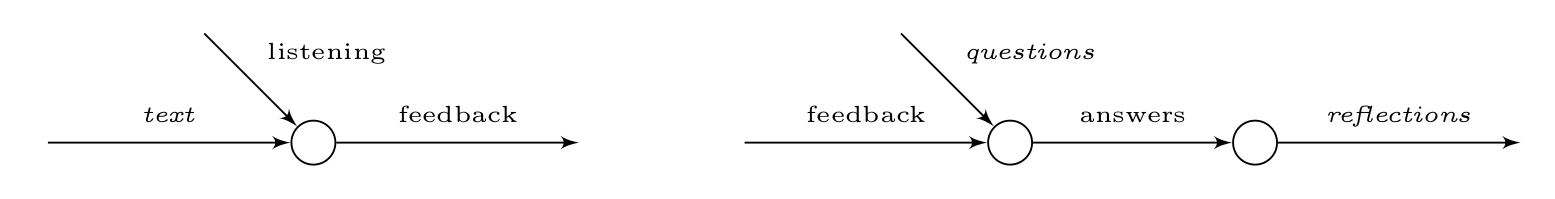
\includegraphics[width=.9\textwidth]{ww-serendipity-diagram}
%% \par}

Italicised elements (\emph{presentation}, \emph{questions}, and
\emph{reflections}) are the responsibilities of the presenting author,
and the upright elements (listening, feedback, and
answers) are the responsibilities of the attendant critics.
%
The system as a whole can be further decomposed into generative
components as follows:

\bigskip

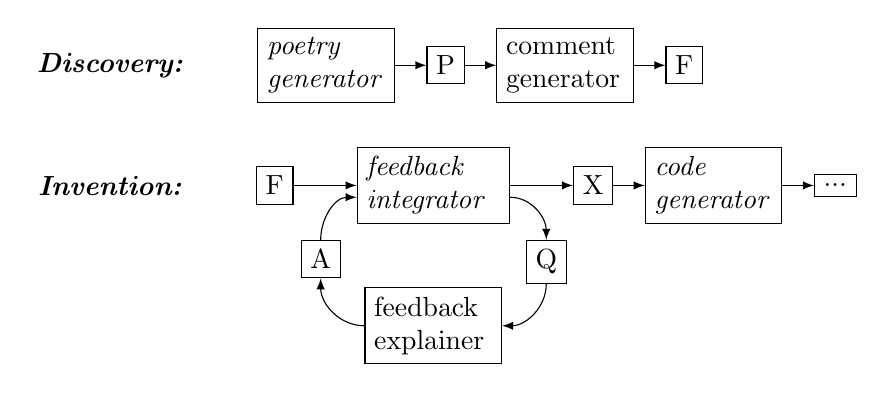
\begin{tikzpicture}[
single/.style={draw, anchor=text, rectangle},
]
\node (discovery) {\textbf{\emph{Discovery:}}};
% poet generates poem
\node[single, right=8mm of discovery.east,text width=1.5cm] (poet) {\emph{poetry generator}};
\node[single, right=4mm of poet.east] (poem) {P};
\draw [-latex] (poet.east) -- (poem.west);
% critic listens to poem and offers feedback
\node[single, right=4mm of poem.east,text width=1.5cm] (critic) {comment generator};
\draw [-latex] (poem.east) -- (critic.west);
\node[single, right=4mm of critic.east] (feedback) {F};
\draw [-latex] (critic.east) -- (feedback.west);

%%% Next phase
\node[below=1cm of discovery] (invention) {\textbf{\emph{Invention:}}};
% poet integrates feedback
\node[single, right=8mm of invention.east] (feedbackcont) {F};
\node[single, right=8mm of feedbackcont.east,text width=1.7cm] (integrator) {\emph{feedback integrator}};
\draw [-latex] (feedbackcont.east) -- (integrator.west);

\node[single, below=8mm of integrator.south,text width=1.5cm] (explainer) {feedback explainer};

\node[single, below right=2mm and 2mm of integrator] (question) {Q};
\node[single, below left=2mm and 2mm of integrator] (answer) {A};

\draw[-latex] ([yshift=-1.5mm]integrator.east) to [out=0,in=90] (question.north) ;
\draw[-latex] (question.south) to [out=270,in=0] (explainer.east) ;
\draw[-latex] (explainer.west) to [out=180,in=270] (answer.south) ;
\draw[-latex] (answer.north) to [out=90,in=180] ([yshift=-1.5mm]integrator.west) ;

\node[single, right=8mm of integrator.east] (problem) {X};

\draw [-latex] (integrator.east) -- (problem.west);

% poet reflects on feedback and updates codebase

\node[single, right=4mm of problem.east,text width=1.5cm] (pgrammer) {\emph{code}\\ \emph{generator}};

\draw [-latex] (problem.east) -- (pgrammer.west);

\node[single, right=4mm of pgrammer.east,text width=.3cm] (etc) {...};

\draw [-latex] (pgrammer.east) -- (etc.west);
\end{tikzpicture}


\bigskip

\noindent In our thought experiment, we focus on the case of hypothetical such discussions and exchange of views between computational poetry systems as our example of a situation where social circumstances could encourage serendipity. We note that similar
ideas would apply for prose and, with further adaptation, other arts.

\paragraph{Thought Experiment: Prepared mind.}
Participating systems need to be able to follow the protocol.  This
means that participating systems will need components like those
listed above. The {\tt listening} and {\tt questions} components of
the protocol correspond to $p$ and $p^{\prime}$ our model of
serendipity.  The corresponding ``comment generator'' and ``feedback
integrator'' modules in the architecture represent the primary points
of interface to the outside world.  In principle these modules need to
be prepared to deal (more or less thoughtfully) with \emph{any} text,
and in turn, with \emph{any} comment on that text.  Certain limits may
be agreed in advance; e.g.~as to genre or length in the case of texts,
and what constitutes an acceptable comment.  The ``feedback
explainer'' is closely connected with the ``comment generator'' and in
an implementation of this model they would presumably share a
codebase.  The loop for learning by asking questions as they arise is
reminiscent of the operating strategy of {\sf SHRDLU}
\cite{winograd1972understanding}.

\paragraph{Thought Experiment: Serendipity triggers.}

Although the poem is under the control of the initial generative
subsystem, it is \emph{not} under control of the listening subsystem.
The listening subsystem expects some poem, but it does not know what
poem to expect.  In this sense, the poem constitutes a serendipity
trigger $T$, not only for the listening subsystem, but for the
Workshop system as a whole.

To expand this point, note that there may be several listeners, each
sharing their own feedback and listening to the feedback presented by
others (which, again, is outside of their direct control).  This
creates further potential for serendipity, since each listener can
learn what others see in the poem.  More formally, in this case
$T^\star$ may seen as an evolving vector with shared state, but viewed
and handled from different perspectives.  With multiple agents
involved in the discussion, the ``comment generator'' module would
expand to contain its own feedback loops.

\paragraph{Thought Experiment: Bridge.}

Feedback on portions of the poem may lead the system to identify new
problems, indeed, new \emph{types} of problems that it hadn't
considered before.  The most immediately feasible case is one in which
the critic is a programmer who can directly program new concepts into
the computer \cite<cf.>{winograd1972understanding}.  However, it would
be hard to call that ``serendipity.''

We can also ask whether agents can build new concepts \emph{without}
outside intervention, starting with some basic concepts and abilities
related to poetry (e.g.~definitions of words, valence of sentiments,
metre, repetition, density, etc.) and code (e.g.~the data, functions,
and macros in which the poetic concepts and workshop protocols are
embodied).  Previous experiments with concept invention have been
fraught with questions about autonomy
\cite{ritchie1984case,lenat1984and}.  One cognitively inspired
hypothesis is that the formation of new concepts is closely related to
formation of sensory experiences \cite{milan2013kiki}.  If the
workshop participants have the capacity to identify the distinctive
features of a given poem, then training via a machine learning or
genetic algorithm approach could be used assemble a battery of
existing low-level tools that can approximate the effect.  Relatedly,
a compression process could seek to produce a given complex poetic
effect with a maximally-succinct algorithm.

The key point is that feedback on the poem -- simply describing what's
in the poem from several different points of view -- can be used to
define new problems for the system to solve.  This is not simply a
matter of decomposing the poem into pieces, but also of reconstructing
the way in which the pieces work together.  This is one of the
functions of the {\tt questions} step corresponding to $p^{\prime}$ in
our formalism: they offer the poet the opportunity to enquire about
how different pieces of feedback fit together, and learn more about
where they come from.  Although computers are currently nowhere close,
the reconstructive process may steadily approach the ideal case --
familiar to humans -- of relating to the sentiment expressed by the
poem as a whole \cite[p. 209]{bergson1983creative}.

%% Several of us are involved with a contemporary project
%% \cite{coinvent14} to develop a formal theory of concept invention,
%% focusing on \emph{concept blending}.  The additive or subtractive
%% blending of existing poetry profiles may be another way to create new
%% concepts.


%% should be possible Modifer Grammar
%% Counting Breathing Position Distribution Phonics Rhythm Repetition
%% Thematic Narrative Entropy

\paragraph{Thought Experiment: Result.} 

The final step is to take the problem or problems that were
identified, and write new code to solve them.  Several strategies for
generating a result $R$, in the form of new code, were described
above.  Now the system evaluates the new code to see whether it holds
promise.  In order to do this, it must have a way to carry out an
evaluation and judge whether $|R|>0$.  In the most straightforward
case, it would simply make changes to the draft poem that seem to
improve it in some way.  For example, the poet might remove or alter material that
elicited a negative response from a critic.  The system may proceed to
update its modules related to poetry generation.  Notably, it may also update its own
feedback modules, after reflecting on questions like: ``How might the
critic have detected that feature in my poem?''

We then develop several case studies (some historical and some imagined) showing
how serendipitous discovery+invention can work in a computational setting.
% 
\section{Discussion} \label{sec:discussion}

\subsection{Recommendations} \label{sec:recommendations}

In the diagrammatic formalism advanced in
\cite{colton-assessingprogress}, we spoke about progress with
\emph{systems} rather than with \emph{problems}.  It would be a useful
generalisation of the formalism -- and not just a simple relabelling
-- to tackle problems as well.
%
Figueiredo and Campos \cite{Figueiredo2001}, for example, describe
serendipitous ``moves'' from one problem to another.
%
However, progress with problems does not always mean transforming a
problem that cannot be solved into one that can.  Progress may also
apply to growth in the ability to posit problems.  As Deleuze writes:
``True freedom lies in the power to decide, to constitute problems
themselves'' \cite[p. 15]{deleuze1991bergsonism}.  Indeed, against any
education by means of ready-made problems, Dewey's perspective was
that
\begin{quote}
``\emph{the child's mind can be trained only in so far as the objects
    with which they are occupied arise out of their interests and
    their own problems.}''~\cite{dewey-by-mead}
\end{quote}

This was our emphasis in Section \ref{sec:unified-approach}:
developing new design patterns is closely connected with -- and in the
dynamical interpretation we prefer, effectively synonymous with --
positing new problems.  Although \cite{colton-assessingprogress}
presented a way to model creative progress at various levels of
granularity, it dealt primarily with \emph{solutions}; and although it
exhibited progress in a way that would be recognised by impartial
observers, the formalism did not focus on expositing the features that
would permit a system to actually \emph{make} creative progress.
Accordingly, we would recommend that in applying our earlier
formalism, system designers clearly record what problem a given system
solves, and the degree to which the computer was responsible for
coming up with this problem.

In \cite{stakeholder-groups-bookchapter}, we advanced a broader
programme for computational creativity, in which we argue in favour of
studying the \emph{perceptions} of creativity by various parties.  The
criteria developed in the current paper -- including the focus shift,
which we regard as fundamental -- can be used in the same way, as we
will describe below.

%% MC> Angelina is a able to read Twitter to find out what people think of
%% MC> people like Hamid Karzai, and then change the sorts of images that
%% MC> it finds as a result.  So you're going to see a happy picture of
%% MC> President Obama later next to a very angry picture of Hamid Karzai.
%% MC> While some of this might look creative and intelligent, a lot of it
%% MC> comes down to serendipity as well.  So the image you're about to see
%% MC> comes up for a Google search for terrorism that doesn't really have
%% MC> much relevance to the news article, and the sound that you're
%% MC> hearing now, the electronic drone, sounds like it's a good choice
%% MC> for a game that's about war and about feeling unsettling.  But in
%% MC> actuality I have no idea how Angelina came up with that choice.

Our proposed Writers Workshop is very different from the Turing-style
imitation game, but nevertheless may prove to be a useful aptitude
test for computer systems, and as a context in which computationally
creative programs may become aware of each other, and participate
actively in advancing the field of research.  We previously examined
perceptions of creativity in computational systems found among members
of the general public, Computational Creativity researchers, and
creative communities -- understood as human communities.  We should
now add a fourth important ``stakeholder'' group in computational
creativity research: computer systems themselves.

To make the point emphatically: the writers workshop proposed above is
very different from a traditional system ``Show and Tell'' presented
by system developers, for system developers.  Traditional academic
practices associated with presenting finished work, or even
work-in-progress, are not entirely suitable for the field of
computational creativity, where engagement between systems may exhibit
manifestly serendipitous results.  If the community does not implement
a suggestion like the one presented here, it will be missing out on a
key idea for enhancing computational creativity that has been
circulating since Turing suggested that computers should ``be able to
converse with each other to sharpen their wits''
\cite{turing-intelligent}.  Other fields, including computer Go
\cite{bouzy2001computer} and argumentation \cite{yuan2008towards} have
their own dedicated servers and protocols for exchange.  We should
move in that direction too.

There is ample room for unpredictability in such pursuits.  Creativity
may look very different to this fourth stakeholder group than it looks
to us.  In time to come, computer systems will increasingly take
leadership in matters of genre, interaction design, and their own
artistic and scientific training.  For now, our job is not at all to
get out of the way, like the parents of young adults, but rather to
participate in creating the ``play schools'' in which systems that are
quite frankly in early development can begin to socialise with each
other.
%
In \cite{stakeholder-groups-bookchapter}, we introduced nine
hypotheses related to the perception of creativity in computational
systems. 
The last of these hypotheses stated that:
\begin{quote}
``\emph{The perception of creativity in software which produces
  artefacts within a creative community will be increased if the
  software can exhibit subjective judgements about its own work and
  that of others, and defend those judgements in an accountable
  way.}''~\cite{stakeholder-groups-bookchapter}
\end{quote}
If the framework described in this paper is developed further, we may
be able to test this hypothesis in computer simulations.

Our proposed template for design patterns for participation in writers
workshops is different from, but complementary to Alexander's
framework.  Whereas Alexander focused on solutions to common
architectural problems (\emph{A place to wait}, etc.), our framework
is primarily designed to elicit and engage with new and unexpected
problems.  We presented four examples using the template, but our
intention is for the template to be used in a reflective mode by
systems to generate new patterns, in a manner appropriate to
second-order cybernetics.  Many practical issues remain to be settled
for a future computational enterprise that seeks to combine existing
design patterns and new stimuli in order to generate new, useful
design patterns.  One thing that becomes clear from this discussion is
that \emph{problem-setting} is a fundamental issue for the field of
computational creativity that will only be given due attention when
the research culture is ready to fully embrace serendipity.

\begin{quote}
``[S]\emph{ocial cybernetics must be a second-order cybernetics--a
    cybernetics of cybernetics--in order that the observer who enters
    the system shall be allowed to stipulate his own purpose: he is
    autonomous.}'' \cite[p. 286]{von2003essays}
\end{quote}

\subsection{Future Work} \label{sec:futurework}

From this, we extract recommendations for practitioners in computational creativity, and outline our own plan of work.
% \section{Conclusion} \label{sec:conclusion}

%
We began by surveying ``serendipity'', developing a broad historical
view, and describing several criteria for serendipity which we propose
to be computationally salient.  We reviewed related work; like
\citeA{andre2009discovery}, we propose a two-part definition of
serendipity: \emph{discovery} followed by \emph{invention}.
%
Adapting the ``Standardised Procedure for Evaluating Creative
Systems'' (SPECS) model from \citeA{jordanous:12}, we developed a set
of evaluation standards for serendipity.
%
We used this model to analyse prior examples of serendipity in the
context of evolutionary music improvisation and recommender systems,
and developed a thought experiment that seems able to support ``high
serendipity'' with a novel design for a computational poetry workshop.
%
We then reflected back over our definition, outlining a programme for
serendipitous computing in the pursuit of \emph{autonomy},
\emph{learning}, \emph{sociality}, and \emph{embedded evaluation}.  We
posit the following challenges, which connect with ongoing discussions
in the field:
%
\begin{itemize}
\item \emph{A primary challenge to the serendipitous operation of
  computers is developing computational agents that specify their own
  problems.}
\item \emph{A second challenge is for computational agents to learn
  more and more about the world we live in.}
\item \emph{A third challenge is for computational agents to interact
  in a recognisably social way with us and with each other, resulting
  in emergent effects.}
\item \emph{A fourth challenge is for computational agents to evaluate
  their own creative process and products.}
\end{itemize}
%
In the current work, we have limited ourselves to clarifying
conceptual issues surrounding our definition of serendipty, and
examining their design implications.
% 
We indicate several possible further directions for implementation
work in each of our case studies.  We have also drawn attention to
theoretical questions related to doing program design in an autonomous
programming context.  Our examples show that serendipity is not
foreign to computing practice.  There are further gains to be had for
research in computing by planning -- and programming -- for
serendipity.
%


\\[.5cm]
%
%% \keywords{serendipity,
%% design patterns,
%% intelligent machinery,
%% Writers Workshops}
\end{abstract}


\tableofcontents

\newpage

\section{Introduction}

Although computational creativity is well studied in both theory and
practice, the role of \emph{serendipity} has often not been discussed
in this field -- even though serendipity has played a well-documented
role in historical instances of scientific and technical creativity.
One reason for this omission may be that the field of computational
creativity has tended to focus on artistic creativity.  But
serendipity is increasingly seen as relevant within the arts
\cite{mckay-serendipity} and other creative enterprises
\cite{kakko2009homo,engineering-serendipity}: it is managed and
encouraged with methods ranging from architecture to data science.
%
An interdisciplinary perspective on the phenomenon of serendipity
promises further illumination.  Here, we consider the potential for
formalising this concept and investigate its utility as a new
framework for computational creativity.

Serendipity centres on reassessment.  For example, a non-sticky
``superglue'' that no one was quite sure how to use turned out to be
just the right ingredient for 3M's Post-it\texttrademark\ notes.
%
Serendipity is related, firstly, to deviations from expected or
familiar patterns, and secondly, to new insight.
%
When we consider the practical uses for weak glue, the possibility
that a life-saving antibiotic might be found growing on contaminated
petri dishes, and or the idea that cockle-burs could be anything but
annoying, we encounter radical changes in the evaluation of what's
interesting.  In the \emph{d\'enouement}, what was initially
unexpected is found to be both explicable and useful.

Van Andel \citeyear{van1994anatomy} -- echoing Poincar\'e's
\citeyear{poincare1910creation} (negative) reflections on the potential
for a purely computational approach to mathematics -- claimed that:
\begin{quote}
``\emph{Like all intuitive operating, pure serendipity is not amenable
    to generation by a computer.  The very moment I can plan or
    programme `serendipity' it cannot be called serendipity
    anymore}.'' \cite{van1994anatomy}
\end{quote}
We believe that serendipity is not so mystical as such statements
might seem to imply, and in Section \ref{sec:discussion} we indicate
van Andel's ``patterns of serendipity'' are likely to be highly
applicable in computational settings.

First, in
Section \ref{sec:literature-review}, we survey the broad literature on
serendipity. Then in Section \ref{sec:background} we present our formal
definition of serendipity, and examine related work that has applied
the concept of serendipity in a computational context. Section \ref{sec:connections-to-formal-definition} makes connections from historical examples of
serendipitous discovery and invention to our formal model.  Section
\ref{sec:computational-serendipity} then presents case studies and
thought experiments in terms of this model.  Section
\ref{sec:discussion} offers recommendations for researchers working in
computational creativity (a key research area concerned with the computational modelling of serendipity), and describes our own plans for future
work.  Section \ref{sec:conclusion} reviews the argument and
summarises the limitations of our analysis.




%% The literature review
\section{Literature review} \label{sec:literature-review}

In this section, we give a short overview covering the etymology of
the term ``serendipity'' and trace its development in order to pin
down the key commonalities from many definitions and instances.  In
particular, we point out key conditions of serendipity, their
components and general characteristics, including environmental
factors.  The structure of this section follows and updates an earlier
survey from \citeA{pease2013discussion}, drawing connections with our
formal model described above.

\subsection{Etymology and selected definitions} \label{sec:overview-serendipity}
The English term ``serendipity'' derives from the 1302 long poem \emph{Eight Paradises}, written in Persian by the Sufi poet Am\={\i}r Khusrow in Uttar Pradesh.\footnote{\url{http://en.wikipedia.org/wiki/Hasht-Bihisht}}  In the English-speaking world, its first chapter became known as ``The Three Princes of Serendip'', where ``Serendip'' represents the Old Tamil-Malayalam word for Sri Lanka (%{\tam சேரன்தீவு},
\emph{Cerantivu}), ``island of the Ceran kings.''

The term ``serendipity'' is first found in a 1757 letter by Horace Walpole to Horace Mann:
\begin{quote}
\emph{``This discovery is almost of that kind which I call serendipity, a very expressive
word} \ldots \emph{You will understand it better by the derivation than by the
definition. I once read a silly fairy tale, called The Three Princes of Serendip:
as their Highness travelled, they were always making discoveries, by accidents
\& sagacity, of things which they were not in quest of}[.]''~\cite[p. 633]{van1994anatomy}
\end{quote}
The term became more widely known in the 1940s through studies of serendipity as a factor in scientific discovery, surveyed by Robert Merton and Elinor Barben \citeyear{merton} in their 1957 analyis ``The Travels and Adventures of Serendipity, A Study in Historical Semantics and the Sociology of Sciences''.  Merton and Barben define the term as follows:
\begin{quote}
\emph{``The serendipity pattern refers to the fairly common experience of observing
an unanticipated, anomalous and strategic datum which becomes the occasion
for developing a new theory or for extending an existing theory.''} \cite[p. 635]{van1994anatomy}
\end{quote}
In 1986, Philippe Qu\'eau described serendipity as ``the art of
finding what we are not looking for by looking for what we are not
finding'' \cite{eloge-de-la-simulation}, as quoted in
\cite[p. 121]{Campos2002}.  Pek van Andel
\citeyear[p. 631]{van1994anatomy} describes it simply as ``the art of
making an unsought finding''.


Roberts \citeyear[pp. 246--249]{roberts} records 30 entries for the term ``serendipity'' from English language dictionaries dating from 1909 to 1989.  
%
Classic definitions require the investigator not to be aware of the problem they serendipitously solve, but this criterion has largely dropped from dictionary definitions. Only 5 of Roberts' collected definitions explicitly say ``not sought for.''  Roberts characterises ``sought findings'' in which an accident leads to a discovery with the term \emph{pseudoserendipity} \cite{chumaceiro1995serendipity}.
%
While Walpole initially described serendipity as an event, it has
since been reconceptualised as a psychological attribute, a matter of
sagacity on the part of the discoverer: a ``gift'' or ``faculty'' more
than a ``state of mind.''  Only one of the collected definitions, from
1952, defined it solely as an event, while five define it as both
event and attribute.

However, there are numerous examples that exhibit features of
serendipity which develop on a social scale rather than an individual
scale.  For instance, between Spencer Silver's creation of high-tack,
low-adhesion glue in 1968, the invention of a sticky bookmark in 1973,
and the eventual launch of the distinctive canary yellow re-stickable
notes in 1980, there were many opportunities for
Post-its\texttrademark\ \emph{not} to have come to be
\cite{tce-postits}. Accordingly, Merton and Barber argue that the
psychological perspective needs to be integrated with a
\emph{sociological} one.\footnote{ ``For if chance favours prepared
  minds, it particularly favours those at work in microenvironments
  that make for unanticipated sociocognitive interactions between
  those prepared minds. These may be described as serendipitous
  sociocognitive microenvironments'' \cite[p. 259--260]{merton}.}
Large-scale scientific and technical projects generally rely on the
``convergence of interests of several key actors''
\cite{companions-in-geography}, along with other supporting cultural
factors.  Umberto Eco \citeyear{eco2013serendipities} focuses on the
historical role of serendipitous mistakes and falsehoods in the
production of knowledge.

It is important to note that serendipity is usually discussed within
the context of \emph{discovery}, rather than \emph{creativity},
although in typical parlance these terms are closely related
\cite{jordanous12jims}.  In our definition of serendipity, we have
made use of Henri Bergson's distinction:
\begin{quote}
``\emph{Discovery, or uncovering, has to do with what already exists,
    actually or virtually; it was therefore certain to happen sooner
    or later.  Invention gives being to what did not exist; it might
    never have happened.}''~\cite{bergson2010creative}
\end{quote}
As we have indicated serendipity would seem to require features of
both; that is, the discovery of something unexpected and the invention
of an application for the same.  We must complement \emph{analysis}
with \emph{synthesis} \cite{delanda1993virtual}.  The balance between
these two features will differ from case to case.

In the next subsection we will review several historical examples.
First, one further point should be made with reference to the ``The
Three Princes of Serendip''.  Prior to Walpole's coinage, this story
had been adapted by Voltaire into an early chapter of \emph{Zadig},
and in turn ``the method of Zadig'' informed subsequent approaches
both to fiction writing and natural science.  This method is rooted
firstly in discovery:

\begin{quote}
``[Zadig] \emph{pry’d into the Nature and Properties of Animals and
    Plants, and soon, by his strict and repeated Enquiries, he was
    capable of discerning a Thousand Variations in visible Objects,
    that others, less curious, imagin’d were all
    alike.}''~\cite[pp. 21--22]{zadig}
\end{quote}

\noindent Secondly, from disparate observations, Zadig is often able
to assemble a coherent picture:
\begin{quote}
\emph{It was his peculiar Talent to render Truth as obvious as
  possible: Whereas most Men study to render it intricate and
  obscure.}~\cite[p. 54]{zadig}
\end{quote}
Similarly, but in reverse, a coherent picture may be reduced to
fragmented pieces each of which may tell a very different story from
the whole.  This is illustrated in Zadig's misadventure with a broken
tablet, in which one fragment of a poem of praise reads as treasonous
provocation.  In describing the various features of serendipity below,
we will draw connections with the schematic diagram presented in
Section \ref{specs-overview}, in order to unfold the multifaceted
notion of serendipity.

\subsection{Connections between prior literature on serendipity and our formal definition} \label{sec:connections-to-formal-definition}

\subsubsection*{Key condition for serendipity}

\begin{itemize}
\item \textbf{Focus shift}: ``\emph{After removing several of the
  burdock burrs (seeds) that kept sticking to his clothes and his
  dog's fur,}~[de Mestral]~\emph{became curious as to how it
  worked. He examined them under a microscope, and noted hundreds of
  `hooks' that caught on anything with a loop, such as clothing,
  animal fur, or hair. He saw the possibility of binding two materials
  reversibly in a simple fashion, if he could figure out how to
  duplicate the hooks and loops.}''~\cite{wiki:velcro}
%
\inlineitem{This corresponds to the identification of $T^\star$, which
  is common to both sides of the diagram.  \citeA{creativity-crisis}
  write that: ``To be creative requires divergent thinking (generating
  many unique ideas) and then convergent thinking (combining those
  ideas into the best result).''  Accordingly $T^\star$ may be thought
  of as an evolving vector of interesting possibilities or ``strategic data'' \cite[p. 507]{merton1948bearing}.  In de
  Mestral's case, the initial idea of a hook-and-loop fastener
  occurred in 1941 -- followed by a full decade of experimentation
  before he was ready to file a patent claim.  }
\end{itemize}

\subsubsection*{Components of serendipity}

\begin{itemize}
\item \textbf{Prepared mind}: 
Fleming's ``prepared mind'' included his focus
on carrying out experiments to investigate influenza as well as his
previous experience that foreign substances in petri dishes can kill
bacteria.  He was concerned above all with the question ``Is there a
substance which is harmful to harmful bacteria but harmless to human
tissue?''  \cite[p. 161]{roberts}.
%%
%
\inlineitem{This corresponds to the prior
  training $p$ and $p^{\prime}$ in our diagram.}
\item \textbf{Serendipity trigger}: The trigger does not directly
  cause the outcome, but rather, inspires a new insight.  It was long
  known by Quechua medics that cinchona bark stops shivering.  In
  particular, it worked well to stop shivering in malaria patients, as
  was observed when malarial Europeans first arrived in Peru.  The
  joint appearance of shivering Europeans and a South American remedy
  was the trigger.  That an extract from cinchona bark can cure and
  can even prevent malaria was subsequently revealed.
%
\inlineitem{This corresponds to the stimulus $T$ in our diagram.}
%%
\item \textbf{Bridge}: These include reasoning techniques, such as
  abductive inference (what might cause a clear patch in a petri
  dish?); analogical reasoning (de Mestral constructed a target domain
  from the source domain of burs hooked onto fabric); and conceptual
  blending (Kekul\'e blended his knowledge of molecule structure with
  his vision of a snake biting its tail).  The bridge may also rely on
  new social arrangements, such as the formation of cross-cultural
  research networks.
%
\inlineitem{This corresponds to the actions based on $p^{\prime}$
  taken on $T^\star$ leading to $R$.}
%%
\item \textbf{Result}: This may be a new product, artefact, process,
  hypothesis, a new use for a material substance, and so on.  The
  outcome may contribute evidence in support of a known hypothesis, or
  a solution to a known problem.  Alternatively, the result may itself
  be a {\em new} hypothesis or problem.  The result may be a
  ``pseudoserendipitous'' in the sense that it was {\em sought}, while
  nevertheless arising from an unknown, unlikely, coincidental or
  unexpected source.  More classically, it is an \emph{unsought}
  finding, such as the discovery of the Rosetta stone.
%
\inlineitem{This corresponds to our $R$.  Note that $R$ may imply
  updates to $p$ or $p^{\prime}$ in further phases of research.}
\end{itemize}

\subsubsection*{Dimensions of serendipity}

Whereas the foregoing items are the central features of the
definition, the following further characterise the circumstances under
which serendipity occurs in practice.

\begin{itemize}
\item \textbf{Chance}: Fleming \citeyear{fleming} noted: ``There are
  thousands of different moulds'' -- and ``that chance put the mould
  in the right spot at the right time was like winning the Irish
  sweep.''
%
\inlineitem{One must assume that relatively few triggers $T^\star$
  that are identified as interesting actually lead to useful results;
  in other words, the process is fallible.}
%%
\item \textbf{Curiosity}: Venkatesh Rao \citeyear{rao2011tempo} refers
  to a \emph{cheap trick} that takes place early on in a narrative in
  order to establish the preliminary conditions of order.  Curiosity
  with can play this role, and can dispose a creative person to begin,
  or to continue, a search into unfamiliar territory.
%
\inlineitem{The prior training $p$ causes interesting features to be
  extracted, even if they are not necessarily useful; $p^{\prime}$
  asks how these features \emph{might} be useful.  }
%%
\item \textbf{Sagacity}: This old-fashioned word is related to
  ``wisdom,'' ``insight,'' and especially to ``taste'' -- and
  describes the attributes, or skill, of the discoverer that
  contribute to forming the bridge between the trigger and the result.
  In many cases, such as an entanglement with cockle-burs, many others
  will have already been in a similar position and not obtained an
  interesting result.  Once a phenomenon has been identified as
  interesting, the disposition of the investigator may lead to a
  dogged pursuit of a useful application or improvement.
%
\inlineitem{Rather than a simple look-up
  rule, $p^{\prime}$ involves creating new knowledge.}
%%
\item \textbf{Value}: Note that the chance ``discovery'' of, say, a
  \pounds 10 note may be seen as happy by the person who finds it,
  whereas the loss of the same note would generally be regarded as
  unhappy.  Positive judgements of serendipity by a third party would
  be less likely in scenarios in which ``One man's loss is another
  man's gain'' than in scenarios where ``One man's trash is another
  man's treasure.''  If possible we prefer this sort of independent
  judgement \cite{jordanous:12}.
%
\inlineitem{The evaluation $|R|>0$ may be carried out ``locally'' (as
  an embedded part of the process of invention of $R$) or ``globally''
  (i.e.~as an external process).  }
\end{itemize}

\subsubsection*{Environmental factors}

\begin{itemize}
\item \textbf{Dynamic world}: Information about the world develops
  over time, and is not presented as a complete, consistent whole.  In
  particular, value may come later.  Van Andel
  \citeyear[p. 643]{van1994anatomy} estimates that in twenty percent
  of innovations ``something was discovered before there was a demand
  for it.''
%
\inlineitem{$T$ (and $T^\star$) appears within a stream of data with
  indeterminacy.  There is a further feedback loop, insofar as
  products $R$ influence the future state.}
%%
\item \textbf{Multiple contexts}: One of the dynamical aspects at play
  may be the discoverer going back and forth between different
  contexts, with different stimuli.  3M employee Arthur Fry sang in a
  church choir and needed a good way to mark pages in his hymn book;
  he happened to have been attending seminars offered by his colleague
  Silver about restickable glue.
%
\inlineitem{This is reflected directly in our model by the difference
  between the ``context of discovery'' involving prior preparations
  $p$, and the ``context of invention'' involving prior preparations
  $p^{\prime}$.  Both of these may be subdivided further.}
%%
\item \textbf{Multiple tasks}: Even within what would typically be
  seen as a single context, a discoverer may take on multiple tasks
  that segment the context into sub-contexts, or that cause the
  investigator to look in more than one direction.  The tasks may have
  an interesting \emph{overlap}, or they may point to a \emph{gap} in
  knowledge.  As an example of the latter, Penzias and Wilson used a
  large antenna to detect radio waves that were relayed by bouncing
  off of satellites.  After they had removed interference effects due
  to radar, radio, and heat, they found residual ambient noise that
  couldn't be eliminated \cite{wiki:cosmic-radiation}.
%
\inlineitem{Both $T$ and $T^\star$ may be multiple, causing an
  individual process to fork into communicating sub-processes that
  involve different skills sets.}
%%
\item \textbf{Multiple influences}: The ``bridge'' from trigger to
  result is often found through a social network, thus, for instance
  Penzias and Wilson only understood the significance of their work
  after reading a preprint by Jim Peebles that hypothesised the
  possibility of measuring radiation released by the big bang
  \cite{wiki:cosmic-radiation}.
%
\inlineitem{The process as a whole may be multiplied out among
  different communicating investigators.}
\end{itemize}

% % \section{Literature review} 

\subsection{Etymology and selected definitions} \label{sec:overview-serendipity}  
The English term ``serendipity'' derives from the 1302 long poem \emph{Eight Paradises}, written in Persian by the Sufi poet Am\={\i}r Khusrow in Uttar Pradesh.\footnote{\url{http://en.wikipedia.org/wiki/Hasht-Bihisht}}  In the English-speaking world, its first chapter became known as ``The Three Princes of Serendip'', where ``Serendip'' represents the Old Tamil-Malayalam word for Sri Lanka (%{\tam சேரன்தீவு},
\emph{Cerantivu}), ``island of the Ceran kings.''

The term ``serendipity'' is first found in a 1757 letter by Horace Walpole to Horace Mann:
\begin{quote}
\emph{``This discovery is almost of that kind which I call serendipity, a very expressive
word} \ldots \emph{You will understand it better by the derivation than by the
definition. I once read a silly fairy tale, called The Three Princes of Serendip:
as their Highness travelled, they were always making discoveries, by accidents
\& sagacity, of things which they were not in quest of}[.]''~\cite[p. 633]{van1994anatomy}
\end{quote}
The term became more widely known in the 1940s through studies of serendipity as a factor in scientific discovery, surveyed by Robert Merton and Elinor Barber \citeyear{merton} in ``The Travels and Adventures of Serendipity, A Study in Historical Semantics and the Sociology of Sciences''.  Merton \citeyear{merton1948bearing} \cite<cited in>[pp. 195--196]{merton} describes a generalised ``serendipity pattern'' and its constituent parts:

\begin{quote}
``\emph{The serendipity pattern refers to the fairly common experience of observing an \emph{unanticipated}, \emph{anomalous} \emph{and strategic} datum which becomes the occasion for developing a new theory or for extending an existing theory.}''~\cite[p. 506]{merton1948bearing} (original emphasis)
    %% The datum [that exerts a pressure for initiating theory] is, first of all, unanticipated. A research directed toward the test of one hypothesis yields a fortuitous by-product, an unexpected observation which bears upon theories not in question when the research was begun.
    %% Secondly, the observation is anomalous, surprising, either because it seems inconsistent with prevailing theory or with other established facts. In either case, the seeming inconsistency provokes curiosity; it stimulates the investigator to "make sense of the datum," to fit it into a broader frame of knowledge....
    %% And thirdly, in noting that the unexpected fact must be "strategic," i. e., that it must permit of implications which bear upon generalized theory, we are, of course, referring rather to what the observer brings to the datum than to the datum itself. For it obviously requires a theoretically sensitized observer to detect the universal in the particular. 
\end{quote}

In 1986, Philippe Qu\'eau described serendipity as ``the art of
finding what we are not looking for by looking for what we are not
finding'' (\citeNP{eloge-de-la-simulation}, as quoted in
\citeNP[p. 121]{Campos2002}).  Pek van Andel
\citeyear[p. 631]{van1994anatomy} describes it simply as ``the art of
making an unsought finding''.


Roberts \citeyear[pp. 246--249]{roberts} records 30 entries for the term ``serendipity'' from English language dictionaries dating from 1909 to 1989.  
%
Classic definitions require the investigator not to be aware of the problem they serendipitously solve, but this criterion has largely dropped from dictionary definitions. Only 5 of Roberts' collected definitions explicitly say ``not sought for.''  Roberts characterises ``sought findings'' in which an accident leads to a discovery with the term \emph{pseudoserendipity} \cite{chumaceiro1995serendipity}.
%
While Walpole initially described serendipity as an event
(i.e., a kind of discovery), it has
since been reconceptualised as a psychological attribute, a matter of
sagacity on the part of the discoverer: a ``gift'' or ``faculty'' more
than a ``state of mind.''  Only one of the collected definitions, from
1952, defined it solely as an event, while five define it as both
event and attribute.

There are numerous examples that exhibit features of
serendipity which develop on a social scale rather than an individual
scale.  For instance, between Spencer Silver's creation of high-tack,
low-adhesion glue in 1968, the invention of a sticky bookmark in 1973,
and the eventual launch of the distinctive canary yellow re-stickable
notes in 1980, there were many opportunities for
Post-it\texttrademark\ Notes \emph{not} to have come to be
\cite{tce-postits}.  Merton and Barber argue that the
psychological perspective needs to be integrated with a
\emph{sociological} one.\footnote{ ``For if chance favours prepared
  minds, it particularly favours those at work in microenvironments
  that make for unanticipated sociocognitive interactions between
  those prepared minds. These may be described as serendipitous
  sociocognitive microenvironments'' \cite[p. 259--260]{merton}.}
Large-scale scientific and technical projects generally rely on the
``convergence of interests of several key actors''
\cite{companions-in-geography}, along with other supporting cultural
factors.  For example, Umberto Eco \citeyear{eco2013serendipities} focuses on the
historical role of serendipitous mistakes and falsehoods in the
production of knowledge.

It is important to note that serendipity is usually discussed within
the context of \emph{discovery}, rather than \emph{creativity},
although in typical parlance these terms are closely related
\cite{jordanous12jims}.  In our definition of serendipity, we have
made use of Henri Bergson's distinction:
\begin{quote}
``\emph{Discovery, or uncovering, has to do with what already exists,
    actually or virtually; it was therefore certain to happen sooner
    or later.  Invention gives being to what did not exist; it might
    never have happened.}''~\cite{bergson2010creative}
\end{quote}
As we have indicated, serendipity would seem to require features of
both; that is, the discovery of something unexpected and the invention
of an application for the same.  We must complement \emph{analysis}
with \emph{synthesis} \cite{delanda1993virtual}.  The balance between
these two features will differ from case to case.

\citeA{creativity-crisis} write that: ``To be creative requires
divergent thinking (generating many unique ideas) and then convergent
thinking (combining those ideas into the best result).''  This is
exemplified by Voltaire's \citeyear{zadig} character Zadig (a figure inspired
in part by the ``The Three Princes of Serendip''\footnote{\citeA[p. 19]{merton}.}) who ``was capable of
discerning a Thousand Variations in visible Objects, that others, less
curious, imagin’d were all alike'' -- and in addition had the
``peculiar Talent to render Truth as obvious as possible: Whereas most
Men study to render it intricate and obscure.''  An example to aspire to!

% \subsection{Serendipity by example} \label{sec:by-example}

In this section, we illustrate the key condition, components,
dimensions, and environmental factors that support serendipity, using
historical examples.  The structure of this section follows and
updates an earlier survey from \citeA{pease2013discussion}.

\subsubsection*{Key condition for serendipity.}

Serendipity relies on a reassessment or reevaluation -- a \emph{focus shift} in which something that was previously uninteresting, of neutral, or even negative value, becomes interesting.

\begin{itemize}
\item \textbf{Focus shift}: George de Mestral, an electrical engineer
  by training, and an experienced inventor, returned from a hunting
  trip in the Alps.  He removed several burdock burrs from his clothes
  and his dog's fur and became curious about how they worked. After
  examining them under a microscope, he realised the possibility of
  creating a new kind of fastener that worked in a similar
  fashion.
% \cite[p. x]{roberts}
\end{itemize}

\subsubsection*{Components of serendipity.}

A focus shift is brought about by the meeting of a \emph{serendipity trigger} and a \emph{prepared mind}.  The next step involves building a \emph{bridge} to a valuable \emph{result}.

\begin{itemize}
\item \textbf{Prepared mind}: 
Fleming's ``prepared mind'' included his focus
on carrying out experiments to investigate influenza as well as his
previous experience that foreign substances in petri dishes can kill
bacteria.  He was concerned above all with the question ``Is there a
substance which is harmful to harmful bacteria but harmless to human
tissue?''  \cite[p. 161]{roberts}.
\end{itemize}

\begin{itemize}
\item \textbf{Serendipity trigger}: The trigger does not directly
  cause the outcome, but rather, inspires a new insight.  It was long
  known by Quechua medics that cinchona bark stops shivering.  In
  particular, it worked well to stop shivering in malaria patients, as
  was observed when malarial Europeans first arrived in Peru.  The
  joint appearance of shivering Europeans and a South American remedy
  was the trigger.  That an extract from cinchona bark can cure and
  can even prevent malaria was subsequently revealed.
\end{itemize}

\begin{itemize}
\item \textbf{Bridge}: These include reasoning techniques, such as
  abductive inference (what might cause a clear patch in a petri
  dish?); analogical reasoning (de Mestral constructed a target domain
  from the source domain of burs hooked onto fabric); and conceptual
  blending (Kekul\'e blended his knowledge of molecule structure with
  his vision of a snake biting its tail).  The bridge may also rely on
  new social arrangements, such as the formation of cross-cultural
  research networks.
\end{itemize}

\begin{itemize}
\item \textbf{Result}: This may be a new product, artefact, process,
  hypothesis, a new use for a material substance, and so on.  The
  outcome may contribute evidence in support of a known hypothesis, or
  a solution to a known problem.  Alternatively, the result may itself
  be a {\em new} hypothesis or problem.  The result may be a
  ``pseudoserendipitous'' in the sense that it was {\em sought}, while
  nevertheless arising from an unknown, unlikely, coincidental or
  unexpected source.  More classically, it is an \emph{unsought}
  finding, such as the discovery of the Rosetta stone.
\end{itemize}

\subsubsection*{Dimensions of serendipity.}

The four components described above have attributes that may be present to a greater or lesser degree.  These are: \emph{Chance} -- how likely was the trigger to appear?; \emph{Curiosity} -- how likely was this trigger to be identified as interesting?; \emph{Sagacity} -- how likely was it that the interesting trigger would be turned into a result?; -- and \emph{Value} (how valuable is the result that is ultimately produced?).

\begin{itemize}
\item \textbf{Chance}: Fleming \citeyear{fleming} noted: ``There are
  thousands of different moulds'' -- and ``that chance put the mould
  in the right spot at the right time was like winning the Irish
  sweep.''
\end{itemize}

\begin{itemize}
\item \textbf{Curiosity}: Venkatesh Rao \citeyear{rao2011tempo} refers
  to a \emph{cheap trick} that takes place early on in a narrative in
  order to establish the preliminary conditions of order.  Curiosity
  with can play this role, and can dispose a creative person to begin,
  or to continue, a search into unfamiliar territory.
\end{itemize}

\begin{itemize}
\item \textbf{Sagacity}: This old-fashioned word is related to
  ``wisdom,'' ``insight,'' and especially to ``taste'' -- and
  describes the attributes, or skill, of the discoverer that
  contribute to forming the bridge between the trigger and the result.
  In many cases, such as an entanglement with burdock burrs, many others
  will have already been in a similar position and not obtained an
  interesting result.  Once a phenomenon has been identified as
  interesting, the disposition of the investigator may lead to a
  dogged pursuit of a useful application or improvement.
\end{itemize}

\begin{itemize}
\item \textbf{Value}: Note that the chance ``discovery'' of, say, a
  \pounds 10 note may be seen as happy by the person who finds it,
  whereas the loss of the same note would generally be regarded as
  unhappy.  Positive judgements of serendipity by a third party would
  be less likely in scenarios in which ``One man's loss is another
  man's gain'' than in scenarios where ``One man's trash is another
  man's treasure.''  If possible we prefer this sort of independent
  judgement \cite{jordanous:12}.
\end{itemize}

\subsubsection*{Environmental factors.}

Finally, serendipity seems to be more likely for agents who experience and participate in a \emph{dynamic world}, who are active in \emph{multiple contexts}, occupied with \emph{multiple tasks}, and who avail themselves of \emph{multiple influences}.

\begin{itemize}
\item \textbf{Dynamic world}: Information about the world develops
  over time, and is not presented as a complete, consistent whole.  In
  particular, \emph{value} may come later.  Van Andel
  \citeyear[p. 643]{van1994anatomy} estimates that in twenty percent
  of innovations ``something was discovered before there was a demand
  for it.''
\end{itemize}

\begin{itemize}
\item \textbf{Multiple contexts}: One of the dynamical aspects at play
  may be the discoverer going back and forth between different
  contexts, with different stimuli.  3M employee Arthur Fry sang in a
  church choir and needed a good way to mark pages in his hymn book;
  he happened to have been attending seminars offered by his colleague
  Silver about restickable glue.
\end{itemize}

\begin{itemize}
\item \textbf{Multiple tasks}: Even within what would typically be
  seen as a single context, a discoverer may take on multiple tasks
  that segment the context into sub-contexts, or that cause the
  investigator to look in more than one direction.  The tasks may have
  an interesting \emph{overlap}, or they may point to a \emph{gap} in
  knowledge.  As an example of the latter, Penzias and Wilson used a
  large antenna to detect radio waves that were relayed by bouncing
  off of satellites.  After they had removed interference effects due
  to radar, radio, and heat, they found residual ambient noise that
  couldn't be eliminated.
\end{itemize}

\begin{itemize}
\item \textbf{Multiple influences}: The ``bridge'' from trigger to
  result is often found through a social network, thus, for instance
  Penzias and Wilson only understood the significance of their work
  after reading a preprint by Jim Peebles that hypothesised the
  possibility of measuring radiation released by the big bang.
\end{itemize}

% \subsection{Related work} \label{sec:related}

An active research community investigating computational models of serendipity exists in the field of information retrieval, and specifically, in recommender systems \cite{Toms2000}. In this domain, \citeA{Herlocker2004} and \citeA{McNee2006} view serendipity as an important factor for user satisfaction, alongside accuracy and diversity.  Serendipity in recommendations variously require the system to deliver an \emph{unexpected} and \emph{useful}, \emph{interesting}, \emph{attractive} or \emph{relevant} item. 
% \cite{Herlocker2004} \cite{Lu2012},\cite{Ge2010}.  
Definitions differ as to the requirement of \emph{novelty}; \citeA{Adamopoulos2011}, for example, describe systems that suggest items that may already be known, but are still unexpected in the current context.  While standardized measures such as the $F_1$-score or the (R)MSE are used to determine the \emph{accuracy} of a recommendation (as very close to what the user is known to prefer), there is no common agreement on a measure for serendipity yet, although there are several proposals \cite{Murakami2008, Adamopoulos2011, McCay-Peet2011,iaquinta2010can}.
  In terms of our model, these systems focus mainly on producing a \emph{serendipity trigger} for the user and in support of discovery, but they include aspects of user modeling which could bring other elements into play, as we will discuss in Section \ref{sec:computational-serendipity}.

Recent work has examined related topics of \emph{curiosity}
\cite{wu2013curiosity} and \emph{surprise} \cite{grace2014using} in
computing.  This latter work seeks to ``adopt methods from the field
of computational creativity [$\ldots$] to the generation of scientific
hypotheses.''  In contrast to the typical application of recommender
systems, this is an example of an effort focused on computational
invention.

Paul Andr{\'e} et al.~\citeyear{andre2009discovery} have examined
serendipity from a design perspective.  Like us, these authors
proposed a two-part model encompassing ``the chance encountering of
information, and the sagacity to derive insight from the encounter.''
According to Andr\'e et al., the first phase is the one that has most
frequently been automated -- but they suggest that computational
systems should be developed that support both aspects.  They
specifically suggest to focus on representational features:
\emph{domain expertise} and a \emph{common language model}.

Although tremendously useful when they are available, these features
are not always enough to account for serendipitious events.  Using the
terminology we introduced earlier, these features seem to exemplify
aspects of the \emph{prepared mind}.  However, as we mentioned above,
the \emph{bridge} is a distinct process that mental preparation can
support, but that it does not necessarily fully determine.  For example, participants in
a poetry workshop may possess a very limited understanding of each
other's aims or of the work they are critiquing, and may as a
consequence talk past one another to a greater or lesser degree --
while nevertheless finding the overall process of participating in the
workshop itself illuminating and rewarding (often precisely because
such misunderstandings elucidate poor communication choices!).
Various social strategies, ranging from Writers Workshops to open
source software, pair programming, and design charettes
\cite[p. 11]{gabriel2002writer} have been developed to exploit similar
emergent effects and to develop \emph{new} shared language.  In
\cite{poetry-workshop}, we investigate the feasibility of using
designs of this sort in multi-agent systems that learn by sharing and
discussing partial understandings.  This earlier paper remains broadly
indicative, however, and the ideas it describes can see considerable
benefit from the more formal thinking we develop in the current work.

\citeA{robot-rendezvous} develop a discussion of serendipitous
rendezvous in a multi-agent system for a graph exploration problem, in
which ``[h]aving more data about their colleagues, better decisions
are made about the potential serendipity path.''  This has some
similarity to the discursive scenario described above, and shows that
\emph{asymmetric partial knowledge} can support serendipitious
findings.  These examples suggest that a distinction between emergent
knowledge of other actors and knowledge about an underlying domain may
be useful -- although the distinction may be less relevant if
the underlying domain itself has dynamic and emergent features.
\emph{Social coordination} among human users of information systems is
a current research topic. \citeA{rubin2010everyday} point out that
naive end users often \emph{talk about} serendiptious occurrences,
which presents another route for research and evaluation.

The {\sf SerenA} system developed by Deborah Maxwell et al.~\citeyear{maxwell2012designing} offers a case study of several of the points discussed above.
This system is designed to support serendipitous discovery for its (human) users
\cite{forth2013serena}.  The authors rely on a process-based model of
serendipity \cite{Makri2012,Makri2012a} that is derived from user
studies, including interviews with 28 researchers, looking for
instances of serendipity from both their personal and professional
lives.  This material was coded along three dimensions:
\emph{unexpectedness}, \emph{insightfulness}, and \emph{value}.  This
research aims to support the process of forming bridging connections
from unexpected encounter to a previously unanticipated but valuable
outcome.  The theory focuses on the acts of \emph{reflection}
that foment both the creation of a bridge and estimates of the
potential value of the result.
%
While this description touches on all of the features of our model, {\sf
  SerenA} largely matches the description offered by Andr{\'e} et
al.~\citeyear{andre2009discovery} of discovery-focused systems, in which
is user experiences an ``aha'' moment and takes the
creative steps to realise the result.  {\sf SerenA}'s primary computational method is to
search outside of the normal search parameters in order to engineer
potentially serendipitous (or at least pseudo-serendipitous)
encounters.
%% Another
%% earlier related example of this sort of system is {\sf Max}, created
%% by Figueiredo and Campos \citeyear{Campos2002}.  The user emailed {\sf
%%   Max} with an existing list of interests and {\sf Max} would return a
%% web page that might also be of interest.  Other systems with similar
%% support for serendipitous discovery involve searching for analogies
%% \cite{Donoghue2002,Donoghue2012}) as well as content \cite{Iaquinta2008}.

In recent joint work \cite{colton-assessingprogress}, we presented a
diagrammatic formalism for evaluating progress in computational
creativity.  It is useful to ask what serendipity would add to this
formalism, and how the result compares with other attempts to
formalise serendipity, notably Figueiredo and Campos's
\citeyear{Figueiredo2001} `Serendipity Equations'.  In this work,
Figueiredo and Campos describe serendipitous ``moves'' from one
problem to another, which transform a problem that cannot be solved
into one that can.  In our diagrammatic formalism, we spoke about
progress with \emph{systems} rather than with \emph{problems}.  It
would be a useful generalisation of the formalism -- and not just a
simple relabelling -- for it to be able to tackle problems as well.
However, it is important to notice that progress with problems does not always mean transforming a
problem that cannot be solved into one that can.  Progress may also
apply to growth in the ability to \emph{posit} problems.  In keeping
track of progress, it would be useful for system designers to record
(or get their systems to record) what problem a given system solves,
and the degree to which the computer was responsible for coming up
with this problem.

As \cite[p. 69]{pease2013discussion} remark, anomaly detection and
outlier analysis are part of the standard machine learning toolkit --
but recognising \emph{new} patterns and defining \emph{new} problems
is more ambitious.  Complex analogies between evolving problems and
solutions form one of the key strategies for teams of human designers
\cite{Analogical-problem-evolution-DCC}.  Kazjon Grace
\citeyear{kaz-thesis} presents one computational model of the creation
of new concepts and interpretations, but this work did include the
ability to create new higher order relationships necessary for complex
analogies.  New patterns and higher-order analogies were considered in
Hofstadter and Mitchell's {\sf Copycat} and the subsequent {\sf
  Metacat}, but these systems operated in a simple and fairly abstract
``microdomain''
\cite{hofstadter1994copycat,DBLP:journals/jetai/Marshall06}.  %% More
%% recent work in this tradition is surveyed in
%% \cite{eric-nichols-thesis}.

The relationship between serendipity and novel problems receives
considerable attention in the current work, since we want to
increasingly turn over responsibility for creating and maintaining a
prepared mind to the machine.


%% Our core definition
\section{Our computational model of serendipity} \label{sec:background}

The \textbf{serendipity trigger} is denoted by $T$.
%
The \textbf{focus shift} takes place with the identification of
$T^\star$, which is common to both the discovery and the invention
phase.  If the process operates in an ``online'' manner, $T^\star$ may
be an evolving vector of interesting possibilities.
%
The \textbf{prepared mind} corresponds to the prior training relevant in each phase, labelled $p$ and $p^{\prime}$ in our diagram.
%
%
The \textbf{bridge} is comprised of the actions based on $p^{\prime}$
that are taken on $T^\star$ leading to the \textbf{result} $R$, which is ultimately given a positive evaluation.



% \begingroup
\tikzset{
block/.style = {draw, fill=white, rectangle, minimum height=3em, minimum width=3em},
tmp/.style  = {coordinate}, 
sum/.style= {draw, fill=white, circle, node distance=1cm},
input/.style = {coordinate},
output/.style= {coordinate},
pinstyle/.style = {pin edge={to-,thin,black}}
}

\begin{tikzpicture}[auto, node distance=2cm,>=latex']
    \node [sum] (sum1) {};
    \node [input, name=pinput, above left=.7cm and .7cm of sum1] (pinput) {};
    \node [input, name=tinput, left of=sum1] (tinput) {};
    \node [input, name=minput, below left of=sum1] (minput) {};
    \node [input, name=minput, right of=sum1] (moutput) {};
    \draw [->] (pinput) -- node{$p$} (sum1);
    \draw [->] (tinput) -- node{\vphantom{{\tiny g}}$T$} (sum1);
    \draw [->] (sum1) -- node{\vphantom{{\tiny g}}$T^{\star}$}  (moutput);
\end{tikzpicture}
\hspace{1cm}
\begin{tikzpicture}[auto, node distance=2cm,>=latex']
    \node [sum] (sum1) {};
    \node [input, name=pinput, above left=.7cm and .7cm of sum1] (pinput) {};
    \node [input, name=tinput, left of=sum1] (tinput) {};
    \node [input, name=minput, below left of=sum1] (minput) {};
    \node [sum, right of=sum1] (sum2) {};
    \node [input, name=minput, right of=sum2] (moutput) {};
    \draw [->] (pinput) -- node{$p^{\prime}$} (sum1);
    \draw [->] (tinput) -- node{\vphantom{{\tiny g}}$T^{\star}$} (sum1);
    \draw [->] (sum1) -- node{\vphantom{{\tiny g}}$R$} (sum2);
    \draw [->] (sum2) -- node{$|R|>0$}  (moutput);
\end{tikzpicture}
\endgroup


{\centering
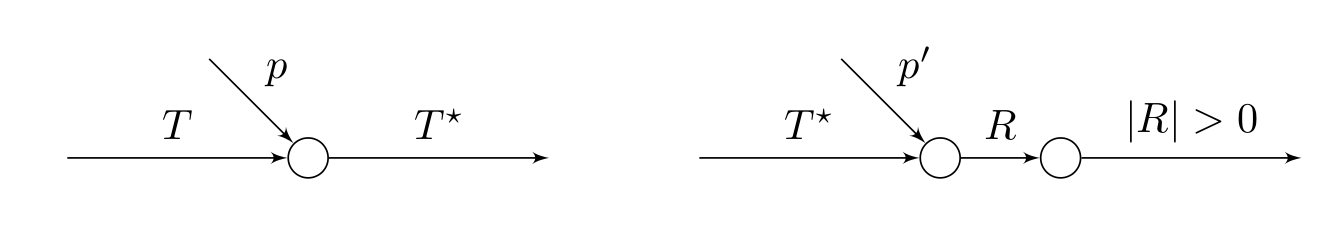
\includegraphics[width=.8\textwidth]{schematic}
\par}


The \textbf{serendipity trigger} is denoted by $T$.
%
The \textbf{focus shift} takes place with the identification of
$T^\star$, which is common to both the discovery and the invention
phase.  If the process operates in an ``online'' manner, $T^\star$ may
be an evolving vector of interesting possibilities.
%
The \textbf{prepared mind} corresponds to the prior training relevant in each phase, labelled $p$ and $p^{\prime}$ in our diagram.
%
%
The \textbf{bridge} is comprised of the actions based on $p^{\prime}$
that are taken on $T^\star$ leading to the \textbf{result} $R$, which is ultimately given a positive evaluation.


The features of our model match and expand upon Merton's \citeyear{merton1948bearing} description of the ``serendipity pattern.'' $T$ is an unexpected observation; $T^\star$ highlights its interesting or anomalous features and recasts them as ``strategic data''; and, finally, the result $R$ may include updates to $p$ or $p^{\prime}$ that inform further phases of research.  

From the point of view of the system under consideration, $T$ is
indeterminate.  Furthermore, one must assume that relatively few of
triggers $T^\star$ that are identified as interesting actually lead to
useful results; in other words, the process is fallible and
\textbf{chance} is likely to play a role.
%
The prior training $p$ causes interesting features
to be extracted, even if they are not necessarily useful; $p^{\prime}$
asks how these features \emph{might} be useful.  These routines 
suggest the relevance of a computational model of \textbf{curiosity}.
%
Far from being a simple look-up rule, $p^{\prime}$ involves creating new knowledge.  A simple example is found in clustering systems, which generate new categories on the fly.  A more complicated example, necessary in the case of updating $p$ or $p^{\prime}$, is automatic programming.  There is a need for \textbf{sagacity} in this sort of affair.
%
Judgment of the \textbf{value} of the result $R$ may be carried out
``locally'' (as an embedded part of the process of invention of $R$)
or ``globally'' (i.e.~as an external process).

As noted, $T$ (and $T^\star$) appears within a stream of data with
indeterminacy.  There is an additional feedback loop, insofar as
products $R$ influence the future state and behaviour of the system.
Thus, the system exists in a \textbf{dynamic world}.
%
Our model separates the
``context of discovery'', involving prior preparations $p$, from the
``context of invention'' involving prior preparations $p^{\prime}$.
Both of these, and the data they deal with, may be subdivided further into \textbf{multiple contexts}. 
%
And correspondingly, since both $T$ and $T^\star$ may be complex, they
may be processed using multiple sub-processes that deal with
\textbf{multiple tasks} using different skills sets.
%
The process as a whole may be multiplied out across different
communicating investigators, so that the final result bears the mark
of \textbf{multiple influences}.





\subsection{Using SPECS to evaluate computational serendipity}\label{specs-overview}

In a 2012 special issue of the journal {\em Cognitive Computation}, on
``Computational Creativity, Intelligence and Autonomy'', Jordanous
analyses current evaluation procedures used in computational
creativity, and provides a much-needed set of customisable evaluation
guidelines, the \emph{Standardised Procedure for Evaluating Creative
  Systems} (SPECS) \cite{jordanous:12}. The three step process of SPECS requires the evaluator to define the concept(s) they are evaluating the system on (originally SPECS was designed to evaluate the concept of creativity). This definition is then converted into testable standards that can be used to evaluate individual systems, or comparatively evaluate multiple systems.

We give a slightly modified version of her earlier evaluation
guidelines, in that rather than attempt a definition and evaluation of
{\em creativity}, we follow the three steps for \emph{serendipity}. 

%\newpage

\subsubsection*{Step 1: A computational definition of serendipity}
\begin{quote} {\em Identify a definition of serendipity that your
    system should satisfy to be considered serendipitous.}\end{quote}

\noindent We adopt the Section \ref{sec:our-model} model as our definition of serendipity for Step 1.
%% This situation can be pictured schematically as follows:


\subsubsection*{Step 2: Evaluation standards for computational serendipity}
\begin{quote} {\em Using Step 1, clearly state what standards you use to evaluate the serendipity of your
    system. }\end{quote}

\noindent Here we need to identify testable standards from our definition of computational serendipity. in other words, we now state the key parts of our definition in a form that can be evaluated as to what degree they are or are not met. 

With our definition in mind, we propose the following standards for evaluating serendipity in computational systems:

%% Serendipity relies on a reassessment or reevaluation -- a \emph{focus shift} in which something that was previously uninteresting, of neutral, or even negative value, becomes interesting.

\begin{description}[itemsep=4pt]
\item[\emph{(\textbf{A - Definitional characteristics})}] \emph{The
  system can be said to have a \emph{\textbf{prepared mind}},
  consisting of previous experiences, background knowledge, a store of
  unsolved problems, skills, expectations, and (optionally) a current
  focus or goal.  It then processes a \emph{\textbf{serendipity
  trigger}} that is at least partially the result of factors outside
  of its control, including randomness or unexpected events.  The
  system then uses reasoning techniques and/or social or otherwise
  externally enacted alternatives to create a \emph{\textbf{bridge}}
  from the trigger to a result.  The \emph{\textbf{result}} is
  evaluated as useful, by the system and/or by an external source.}
\item[\emph{(\textbf{B - Dimensions})}] \emph{Serendipity, and its
  various dimensions, can be present to a greater or lesser degree.
  If the criteria above have been met, we consider the system (and optionally, generate ratings as
  estimated probabilities) along several dimensions:
%
\emph{($\mathbf{a}$ - \textbf{chance})} how likely was this trigger to appear to
  the system?
%
\emph{($\mathbf{b}$ - \textbf{curiosity})} On a population basis, comparing
  similar circumstances, how likely was the trigger to be identified
  as interesting?
%
\emph{($\mathbf{c}$ - \textbf{sagacity})} On a population basis, comparing
  similar circumstances, how likely was it that the trigger
  would be turned into a result?
%
Finally, we ask, again, comparing similar results where possible:
\emph{($\mathbf{d}$ - \textbf{value})} How valuable is the result that
is ultimately produced?}

\medskip

\emph{Then aggregating $\mathbf{a}\times\mathbf{b}\times\mathbf{c}$ gives a
  likelihood score: low likelihood $\mathbf{a}\times\mathbf{b}\times\mathbf{c}$ and high value $\mathbf{d}$ are the criteria we use to say that the event was ``highly serendipitous.''}

\item[\emph{(\textbf{C - Factors})}] \emph{Finally, if the criteria
  from Part A are met, and if the event is deemed ``highly
  serendipitous'' according to the criteria in Part B, then in order
  to deepen our qualitative understanding of the serendipitous
  behaviour, we ask: To what extent does the system exist in a
  \emph{\textbf{dynamic world}}, spanning \emph{\textbf{multiple
      contexts}}, featuring \emph{\textbf{multiple tasks}}, and
  incorporating \emph{\textbf{multiple influences}}?}
\end{description}

\subsubsection*{Step 3: Testing our serendipitous system}

\begin{quote} {\em Test your serendipitous system against the standards stated in Step 2 and report the
results.}\end{quote}

\noindent We will develop several examples of the application of this framework
to examples from computing in Section
\ref{sec:computational-serendipity}.  

\paragraph{Example.}
To get a feel for the likelihood score, briefly consider the case of
de Mestral's invention of Velcro\texttrademark.  There is a
\emph{high} chance of encountering burrs while out walking, but
\emph{very few} of de Mestral's contemporaries would have thought to
investigate them under a microscope, and furthermore even among the
scientifically minded \emph{very few} would conceive of a useful
application or have the perseverance required to carry out the
associated product development.  Hook-and-loop fasteners are now
widely used; and we can call the invention ``highly serendipitous.''



% SPECS-begins.tex
% figures/schematic/schematic.png
% SPECS-continues.tex

%% Development of the idea with examples
\section{Serendipity in computational systems} \label{sec:computational-serendipity}

The 13 criteria from Section \ref{sec:literature-review} specify the
conditions and preconditions that are conducive to serendipitous
discovery.  These criteria have been further formalised
in Section \ref{specs-overview}.
% 
\citeA{pease2013discussion} used a slightly different version of the
SPECS criteria to discuss three examples of serendipitous behaviour:
in dynamic investigation problems, model generation, and poetry
flowcharts.  Two additional examples using the revised criteria are
described below.  These example serve the purpose of illustrating our
revised criteria, and also show forays of computational intelligence
into domains known for serendipity in their everyday cultural context.
We then turn to a more elaborated thought experiment that evaluates
these ideas in the course of developing a new system design.

% \subsection{Proposed experiment: A Writers Workshop for Systems} \label{sec:writers-workshop}

Richard Gabriel \cite{gabriel2002writer} describes the practise of
Writers Workshops that has been put to use for over a decade within
the Pattern Languages of Programming (PLoP) community.  The basic
style of collaboration originated much earlier with groups of literary
authors who engage in peer-group critique.  Some literary workshops
are open as to genre, and happy to accommodate beginners, like the
Minneapolis Writers
Workshop\footnote{\url{http://mnwriters.org/how-the-game-works/}};
others are focused on professionals working within a specific genre,
like the Milford Writers
Workshop\footnote{\url{http://www.milfordsf.co.uk/about.htm}}.  The
practices that Gabriel describes are fairly typical.  Authors come
with work ready to present, and read a short sample, which is then
discussed and constructively critiqued by attendees.  Presenting
authors are not permitted to rebut these comments.  The commentators
generally summarise the work and say what they have gotten out of it,
discuss what worked well in the piece, and talk about how it could be
improved.  The author listens and may take notes; at the end, he or
she can then ask questions for clarification.  Generally, non-authors
are either not permitted to attend, or are asked to stay silent
through the workshop, and perhaps sit separately from the
participating authors/reviewers.  There are similarities between the
Writers Workshops and classical practices of group composition
\cite{jin1975art} and dialectic \cite{dialectique}, and the workshop
may be considered an artistic or creative space in its own right.

In PLoP workshops, authors present design patterns and pattern
languages, or papers about patterns, rather than more traditional
literary forms like poems, stories, or chapters from novels.  Papers
must be workshopped at a PLoP or EuroPLoP conference in order to be
considered for the \emph{Transactions on Pattern Languages of
  Programming} journal.  A discussion of writers workshops
in the language of design patterns is presented by
Coplien and Woolf \cite{coplien1997pattern}.  Their patterns include:
\begin{center}
{\small
\begin{tabular}{l@{\hspace{.2cm}}l@{\hspace{.2cm}}l}
\emph{Open Review} & \emph{Safe Setting} & \emph{Workshop Comprises Authors} \\
\emph{Authors are Experts} & \emph{Community of Trust} & \emph{Moderator Guides the Workshop} \\
\emph{Thank the Author} & \emph{Selective Changes} & \emph{Clearing the Palate} \\
\end{tabular}
}
\end{center}

We propose that a similar pattern-based approach should be deployed
within the Computational Creativity community to design a workshop in
which the participants are computer systems instead of human authors.
The annual International Conference on Computational Creativity
(ICCC), now entering its sixth year, could be a suitable venue.
Rather than the system's creator presenting the system in a
traditional slideshow and discussion, or a system ``Show and Tell,''
the systems would be brought to the workshop and would present their
own work to an audience of other systems, in a Writers Workshop
format.  This might be accompanied by a short paper for the conference
proceedings written by the system's designer describing the system's
current capabilities and goals.  Subsequent publications might include
traces of interactions in the Workshop, commentary from the system on
other systems, and offline reflections on what the system might change
about its own work based on the feedback it receives.  As in the PLoP
community, it could become standard to incorporate this sort of workshop
into the process of peer reviewing journal articles for the new \emph{Journal of
  Computational Creativity}\footnote{\url{http://www.journalofcomputationalcreativity.cc}}.

\begin{table}[p]
\begin{tabular}{lp{.7\textwidth}}
{\bf\emph{Successful error}} & \\
\emph{Van Andel's example}: & Post-it\texttrademark\ notes \\[.2cm]
{\tt presentation}& Systems should be prepared to share interesting ideas even if they don't know directly how they will be useful.  \\
{\tt listening}   & Systems should listen with interest, too. \\
{\tt feedback}    & Even interesting ideas may not be ``marketable.''\\
{\tt questions}   & How is your suggestion useful? \\
{\tt reflections} & New combinations of ideas take a long time to realise, and many different ideas may need to be combined in order to come up with something useful.\\
\end{tabular}
\bigskip

\begin{tabular}{lp{.7\textwidth}}
{\bf\emph{Side effect}} & \\
\emph{Van Andel's example}: & Nicotinamide used to treat side-effects of radiation therapy proves efficacious against tuberculosis. \\[.2cm]
{\tt presentation}& Systems should use their presentation as an experiment. \\
{\tt listening}   & Listeners should allow themselves to be affected by what they are hearing. \\
{\tt feedback}    & Feedback should convey the nature of the effect.\\
{\tt questions}   & The presenter may need to ask follow-up questions to gain insight. \\
{\tt reflections} & Form a new hypothesis before seeking a new audience. \\
\end{tabular}
\bigskip

\begin{tabular}{lp{.7\textwidth}}
{\bf\emph{Wrong hypothesis}} & \\
\emph{Van Andel's example}: & Lithium, used in a control study, had an unexpected calming effect. \\[.2cm]
{\tt presentation}& How is this presentation interpretable as a (``natural'') control study? \\
{\tt listening}   & Listeners are ``guinea pigs''.\\
{\tt feedback}    & Discuss side-effects that do not necessarily correspond to the author's perceived intent. \\
{\tt questions}   & Zero in on the most interesting part of the conversation.\\
{\tt reflections} & Revise hypotheses to correspond to the most surprising feedback. \\
\end{tabular}
\bigskip

\begin{tabular}{lp{.7\textwidth}}
{\bf\emph{Outsider}} & \\
\emph{Van Andel's example}: & A mother suggests a new hypothesis to a doctor. \\[.2cm]
{\tt presentation}& The presenter is here to learn from the audience. \\
{\tt listening}   & The audience is here to give help, but also to get help.\\
{\tt feedback}    & Feedback will inevitably draw on previous experiences and ideas.\\
{\tt questions}   & What is the basis for that remark?\\
{\tt reflections} & How can I implement the suggestions?\\
\end{tabular}
\vspace{.2cm}
\caption{Reinterpreting patterns of serendipity for use in a computational workshop\label{tab:reinterpret}}
\end{table}

\begin{figure}[t]
\begin{center}
\resizebox{.93\textwidth}{!}{
\StickyNote[2.5cm]{myyellow}{{\LARGE {Interesting idea}} \\[4ex] {Surprise birthday party}}[3.8cm] \StickyNote[2.5cm]{mygreen}{{\Large I heard you say:} \\[4ex] {``surprise''} }[3.8cm]
\StickyNote[2.5cm]{pink}{{\Large Feedback:} \\[4ex] {I don't like surprises}}[3.8cm]
}
\resizebox{.61\textwidth}{!}{
\StickyNote[2.5cm]{myorange}{{\LARGE {Question}} \\[4ex] {Not even a little bit?\ldots}}[3.8cm]
\quad \raisebox{-.2cm}{\StickyNote[2.5cm]{myblue}{{\LARGE Note to self:} \\[4ex] {(Try smaller surprises \\ next time.)}}[3.8cm]}
}
\end{center}
\caption{A paper prototype for applying the \emph{Successful Error} pattern\label{fig:paper-prototype}}
\end{figure}

In order to facilitate this sort of interaction, it would be necessary
for systems to implement a basic protocol related to
%%
\[
\text{
{\tt presentation}, {\tt listening}, {\tt
  feedback}, {\tt questions}, and {\tt
  reflections}.}
\]
%%
This protocol could be thought of as a light-weight template for
creating design patterns that guide system-level participation in the
context specified by Coplien and Woolf's pattern language for writers
workshops.  Table \ref{tab:reinterpret} uses this framework to recast
the four ``perfectly'' serendipitous patterns from van Andel --
\emph{Successful error}, \emph{Side effect}, \emph{Wrong hypothesis},
and \emph{Outsider} -- in a form that may make them useful to
developers preparing to enter their systems into the Workshop.
%
Further guidelines for structuring and participating in traditional
writers workshops are presented by Linda Elkin in
\cite[pp. 201-203]{gabriel2002writer}.  It is not at all clear that
the same ground rules should apply to computer systems.  For example,
one of Elkin's rules is that ``Quips, jokes, or sarcastic comments,
even if kindly meant, are inappropriate.''  Rather than forbidding
humour, it may be better for individual comments to be rated as
helpful or non-helpful.  Again, since serendipitous discovery is an
overarching goal, in the first instance, usefulness and interest might
be judged in terms of the criteria described in Section
\ref{sec:evaluation-criteria}.

We would need a neutral environment that is not hard to develop for:
the {\sf FloWr} system described in Section \ref{sec:foundations}
offers one such possibility.  With this system, the basic operating
logic of the Workshop could be spelled out as a flowchart, and
contributing systems could use flowcharts as the basic medium for
sharing their presentations, feedback, and questions.  Developing
around a process language of this sort partially obviates the need for
participating systems to have strong natural language processing
capabilities.  
%
Post-it\texttrademark\ notes, which have provided us with a useful
example of serendipitous discovery, also provide indicative strategies
from the world of paper prototyping (Figure \ref{fig:paper-prototype}).

Gordon Pask's conversation theory, reviewed in
\cite{conversation-theory-review,boyd2004conversation}, goes
considerably beyond what we have presented here as a simple process
language, although there are structural parallels.  In a basic
Pask-style learning conversation: (0) Conversational participants are
carrying out some actions and observations; (1) naming and recording
what action is being done; (2) asking and explaining why it works the
way it does; (3) carrying out higher-order methodological discussion;
and (4) trying to figure out why unexpected results occured \cite[p. 190]{boyd2004conversation}.

Naturally, variations to the underlying system, protocol, and the
schedule of events should be considered depending on the needs and
interests of participants, and several variants can be tried.  On a
pragmatic basis, if the Workshop proved quite useful to participants,
it could be revised to run monthly, weekly, or
continuously.\footnote{For a comparison case in computer Go, see
  \url{http://cgos.computergo.org/}.}


\subsection{Case Studies: Prior art}

\paragraph{Evolutionary music improvisation systems.}

\citeA{jordanous10} reported a computational jazz improvisation system using genetic algorithms. Genetic algorithms, and evolutionary computing more generally, could encourage computational serendipity. We examine Jordanous's system (later given the name {\em GAmprovising} \cite{jordanous:12}) as a case study for evolutionary computing in the context of our model of computational serendipity: to what extent does GAmprovising model serendipity?

GAmprovising uses genetic algorithms to evolve a population of Improvisors. Each Improvisor is able to randomly generate music based on various parameters such as range of notes to be used, preferred notes to be used, rhythmic implications around note lengths and other musical parameters (see \cite{jordanous10}. These parameters are what defines the Improvisor at any point in evolution. After a cycle of evolution, each Improvisor is evaluated via a fitness function based on Ritchie's criteria \cite{ritchie07} of how creative the Improvisor is. Ritchie's criteria use user-supplied ratings of how novel and how appropriate the music produced by the Improvisor is, to calculate 18 criteria that collectively evaluate how creative a system is. The most successful Improvisors (as deemed by the fitness function) are used to seed a new generation of Improvisors, through crossover and mutation operations.

The GAmprovising system can be said to have a \textbf{prepared mind} through its background knowledge of what musical knowledge to embed in the Improvisors and the evolutionary abilities to evolve Improvisors. A \textbf{serendipity trigger} comes from the combination of the mutation and crossover operations employed in the genetic algorithm, and the user input feeding into the fitness function to evaluate produced music. A \textbf{bridge}, from the genetic algorithm operations and user input, to the result is built by the creation of new Improvisors. The \textbf{results} are the various musical improvisations produced by the fittest Improvisors (as well as, perhaps, the parameters that have been considered fittest).

The likelihood of serendipitous evolution is greatly enhanced by the use of mutation and crossover operations within the genetic algorithm, to increase the diversity of search space covered by the system during evolution. However the \textbf{chance} of any particular Improvisor being discovered is low, given the massive dimensions of the search space.  Interesting developments in evolution would be guided by \textbf{curiosity} through the particular human user identifying Improvisors as interesting at that time. \textbf{Sagacity} is determined by how likely the user is to appreciate the same Improvisor's music (or similar music) over time, as tastes of the user may change. The \textbf{value} of the results are maximised through employing a fitness function.

Evolutionary systems such as GAmprovising necessarily operate in a \textbf{dynamic world} which is evolving continuously and may also be affected by changes in user tastes as they evaluate musical output from Improvisors. The \textbf{multiple contexts} arise from the possibility of having multiple users evaluate the musical output (though this is as yet not implemented formally) or through the user changing their preferences over time. \textbf{Multiple tasks} are carried out by the system including evolution of Improvisors, generation of music by individual Improvisors, capturing of user ratings of a sample of the Improvisors' output, and fitness calculations. \textbf{Multiple influences} are captured through the various combinations of parameters that could be set and the potential range of values for each parameter.

\paragraph{Minimally serendipitous systems}

If applied to a system which could be described as minimally serendipitous at best, and perhaps not at all serendipitous, does our model identify the lack of serendipity?

As example, a spellchecker program identifies spelling errors in text input and optionally can correct spelling automatically. The only situation we can conceive of where serendipity could possibly occur is tenuous; perhaps a suggested correction may be incorrect, but may lead the user to interpret the correction in an unexpected way. In all other aspects that we have considered, spellchecker software would be a decidedly unlikely candidate for harbouring serendipitous opportunities.

The system *** %AARGH how do we begin to do this...! to try and apply our model to a spell checker?Giving up for now. I do think it's worth it, perhaps I'm just a bit tired at this point! Feel free to have a go if you fancy the challenge! AJ

% \paragraph{{[}To add: HR.{]}}

\paragraph{Recommender systems.} 

As discussed in Section \ref{sec:related}, recommender systems are one
of the primary contexts in computing where serendipity is seen to play
a role.  As we noted, these systems mostly focus on discovery.
Nevertheless, certain architectures that also take account of
invention would match all of criteria described by our model.  Here we
draw on the observation that recommender systems not \emph{stimulate}
serendipitous discovery for the user: they also have the task of
\emph{simulating} when this is likely to occur.

A recommendation is typically provided if the system suspects that the
item will be likely to introduce ideas that are close to what the user
knows, but that will be unexpected.  In other words, the system aims
to stimulate serendipity for the user. For example, a museum
recommender service might suggest a colourful medieval painting to a
user who seems to like colourful paintings by the modern artist Keith
Haring.  User behaviour (e.g.~following up on these recommendations)
is outside of the direct control of the system and may serve as a
\textbf{serendipity trigger}, and change the way it makes
recommendations in the future.  The system has a \textbf{prepared
  mind}, including both a \emph{user model} and a \emph{domain model},
both of which can be updated dynamically.  The connections through
which recommendations are made usually happen when the system notices
that elements of the domain have something in common via clustering or
faceting.  A \textbf{bridge} to a new kind of recommendation may be
found if new elements are introduced into the domain which do not
cluster well, or if the user appears to know about different clusters
that do not have obvious connections between them.  The intended
outcome of recommendations depend on the organisational mission
e.g.~to make money, to provide a good user experience, etc.; at the
system level, the serendiptious \textbf{result} would be learning a
new approach that helps to address these goals better.

From the perspective of our model, \textbf{chance} will only have a
significant role when the system has the capacity to learn from user
behaviour.  In fact, Bayesian methods are used in contemporary
recommender systems (surveyed in Chapter 3 of
\citeNP{shengbo-guo-thesis}).  The typical commercial perspective on
recommendations is related to the process of ``conversion'' -- turning
recommendations into clicks and clicks into purchases.  Combined with
the ability to learn, \textbf{curiosity} could be described as the
urge to make ``outside-the-box''\footnote{\citeA{abbassi2009getting}.}
recommendations specifically for the purposes of learning more about
users, possibly to the detriment of other goals over the short term.
Measures of \textbf{sagacity} would relate to the system's ability to
draw inferences from user behaviour that would update the
recommendation model.  For example, the system might do A/B testing to
decide how novel recommendation strategies influence conversion.  The
\textbf{value} of recommendation strategies can be measured in terms
of traditional business metrics or other organisational objectives.

A \textbf{dynamic world} which nevertheless exhibits some regularity
is a precondition for useful A/B testing.  As mentioned above the
primary \textbf{(multiple) contexts} are the user model and the domain
model.  A system matching the description here would have
\textbf{multiple tasks}: making useful recommendations, generating new
experiments to learn about users, and building new models based on the
results of these experiments.  Such a system could avail itself of
\textbf{multiple influences} related to experimental design,
psychology, and domain understanding.

% As a general comment, we would say that this is largely how
% \emph{research and development} of recommender systems works, but
% without the same levels of system automony envisioned here.
\begin{table}[ht]%dp]
\caption{Summary: applying computational serendipity model to positive case studies}
\begin{center}
\footnotesize
\begin{tabular}{|c|l|l|}
\hline
  & Evolutionary music systems & Recommender systems \\
\hline
\hline
%{\em Key Condition}  && \\
%Focus shift && \\
%\hline
{\em Components} && \\
\hline
\hline
Serendipity trigger & Evolutionary operations and user input & Input from user behaviour \\
\hline
Prepared mind  & Musical knowledge, evolution mechanisms & Through user model/domain model \\
\hline
Bridge  & Creation of newly-evolved Improvisors & Elements identified outside clusters \\
\hline
Result & Music generated by fittest Improvisors& Dependent on organisation goals \\
\hline
\hline
{\em Dimensions} && \\
\hline
\hline
Chance & If discovered in huge search space & If learning from user behaviour \\
\hline
Curiosity & If a particular user notes an Improvisor & Making unusual recommendations \\
\hline
Sagacity & User appreciation of Improvisor over time & Updating models after user behaviour \\
\hline
Value & Via fitness function (proxy of creativity) & As per business metrics/objectives \\
\hline
\hline
{\em Environmental} && \\
{\em Factors} && \\
\hline
\hline
Dynamic & Continuous computational evolution& As precondition for testing system's \\
 world & \hspace{3mm}and changes in user tastes & \hspace{3mm} influences on user behaviour\\
\hline
Multiple & Multiple & User model and domain model\\
contexts & \hspace{3mm}users opinions? & \\
\hline
Multiple & Evolving Improvisors, generating music,  & Making recommendations, learning\\
 tasks & \hspace{3mm}collecting user input, fitness calculations& \hspace{3mm}from users, updating models \\
\hline
Multiple & Through various musical& Experimental design, psychology, \\
influences &\hspace{3mm}parameter combinations& \hspace{3mm} domain understanding\\
\hline
\end{tabular}
\end{center}
\label{caseStudies}
\end{table}%
\normalsize

\subsection{Thought experiment:  Serendipity by design} \label{sec:ww}

To further evaluate our computational framework in usage, in this
section we develop a thought experiment in system design, based on a
novel computational scenario where there is high potential for
serendipity.  As discussed above, sociological factors can influence
serendipitous discoveries on a social scale.  In our two case studies,
user input played a significant role.  The exploitation of social
creativity and feedback can create scenarios where serendipity could
occur within a computer system as well.

In \cite{poetry-workshop}, we described the preliminary designs for
multi-agent systems that learn by sharing work in progress and
discussing partial understandings.  
%
Following \citeA{gabriel2002writer}
% we described a template for a pattern
% language for interactions in a computational poetry workshop, closely
we define a \emph{Workshop} to be an activity for two or more agents
consisting of the following steps:
%itemize?
{\tt presentation}, {\tt listening}, {\tt feedback}, {\tt questions},
and {\tt reflections}.  In general, the first and most important
feature of {\tt feedback} is for the listener to say what they heard;
in other words, what they find in the presented work.  In some
settings this is augmented with {\tt suggestions}.  After any {\tt
  questions} from the author, the commentators may make {\tt replies}
to offer clarification.

The key steps map quite conveniently into the schematic description of serendipity that we introduced in Section \ref{sec:our-model}:

\begin{center}
\begingroup
\tikzset{
block/.style = {draw, fill=white, rectangle, minimum height=3em, minimum width=3em},
tmp/.style  = {coordinate}, 
sum/.style= {draw, fill=white, circle, node distance=1cm},
input/.style = {coordinate},
output/.style= {coordinate},
pinstyle/.style = {pin edge={to-,thin,black}}
}

\begin{tikzpicture}[auto, node distance=2cm,>=latex']
    \node [sum] (sum1) {};
    \node [input, name=pinput, above left=.9cm and .9cm of sum1] (pinput) {};
    \node [input, name=tinput, left=2.2cm of sum1] (tinput) {};
    \node [input, name=minput, below left of=sum1] (minput) {};
    \node [input, name=minput, right of=sum1] (moutput) {};
    \draw [->] (tinput) -- node{\vphantom{{\footnotesize g}}{\footnotesize \emph{presentation}~~}} (sum1);
    \draw [->] (pinput) -- node{{\footnotesize listening}} (sum1);
    \draw [->] (sum1) -- node{\vphantom{{\footnotesize g}}{\footnotesize feedback}}  (moutput);
\end{tikzpicture}
\hspace{1cm}
\begin{tikzpicture}[auto, node distance=2cm,>=latex']
    \node [sum] (sum1) {};
    \node [input, name=pinput, above left=.9cm and .9cm of sum1] (pinput) {};
    \node [input, name=tinput, left of=sum1] (tinput) {};
    \node [input, name=minput, below left of=sum1] (minput) {};
    \node [sum, right=1.5cm of sum1] (sum2) {};
    \node [input, name=minput, right of=sum2] (moutput) {};
    \draw [->] (tinput) -- node{\vphantom{{\footnotesize g}}{\footnotesize feedback~~}} (sum1);
    \draw [->] (pinput) -- node{{\footnotesize \emph{questions}}} (sum1);
    \draw [->] (sum1) -- node{\vphantom{{\footnotesize g}}{\footnotesize answers}} (sum2);
    \draw [->] (sum2) -- node{{\footnotesize \emph{reflections}}}  (moutput);
\end{tikzpicture}
\endgroup
\end{center}


% figures/ww-serendipity/ww-serendipity.png
%% {\centering
%% 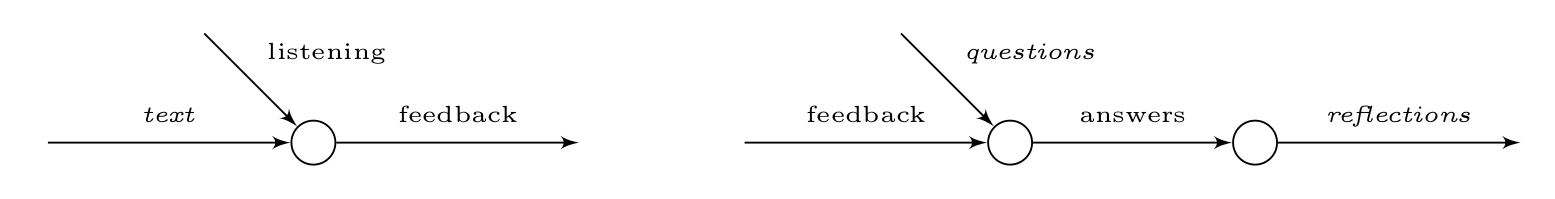
\includegraphics[width=.9\textwidth]{ww-serendipity-diagram}
%% \par}

Italicised elements (\emph{presentation}, \emph{questions}, and
\emph{reflections}) are the responsibilities of the presenting author; the other
elements (listening, feedback, and answers) are the responsibilities of the attendant critics.
%
\begin{figure}
{\centering
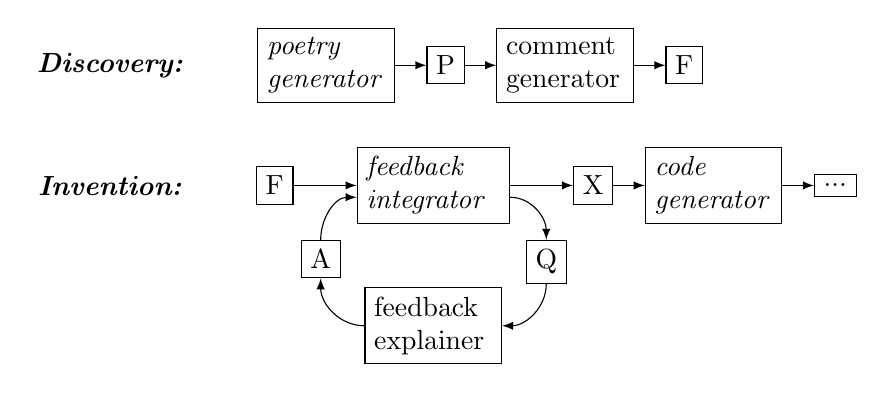
\begin{tikzpicture}[
single/.style={draw, anchor=text, rectangle},
]
\node (discovery) {\textbf{\emph{Discovery:}}};
% poet generates poem
\node[single, right=8mm of discovery.east,text width=1.5cm] (poet) {\emph{poetry generator}};
\node[single, right=4mm of poet.east] (poem) {P};
\draw [-latex] (poet.east) -- (poem.west);
% critic listens to poem and offers feedback
\node[single, right=4mm of poem.east,text width=1.5cm] (critic) {comment generator};
\draw [-latex] (poem.east) -- (critic.west);
\node[single, right=4mm of critic.east] (feedback) {F};
\draw [-latex] (critic.east) -- (feedback.west);

%%% Next phase
\node[below=1cm of discovery] (invention) {\textbf{\emph{Invention:}}};
% poet integrates feedback
\node[single, right=8mm of invention.east] (feedbackcont) {F};
\node[single, right=8mm of feedbackcont.east,text width=1.7cm] (integrator) {\emph{feedback integrator}};
\draw [-latex] (feedbackcont.east) -- (integrator.west);

\node[single, below=8mm of integrator.south,text width=1.5cm] (explainer) {feedback explainer};

\node[single, below right=2mm and 2mm of integrator] (question) {Q};
\node[single, below left=2mm and 2mm of integrator] (answer) {A};

\draw[-latex] ([yshift=-1.5mm]integrator.east) to [out=0,in=90] (question.north) ;
\draw[-latex] (question.south) to [out=270,in=0] (explainer.east) ;
\draw[-latex] (explainer.west) to [out=180,in=270] (answer.south) ;
\draw[-latex] (answer.north) to [out=90,in=180] ([yshift=-1.5mm]integrator.west) ;

\node[single, right=8mm of integrator.east] (problem) {X};

\draw [-latex] (integrator.east) -- (problem.west);

% poet reflects on feedback and updates codebase

\node[single, right=4mm of problem.east,text width=1.5cm] (pgrammer) {\emph{code}\\ \emph{generator}};

\draw [-latex] (problem.east) -- (pgrammer.west);

\node[single, right=4mm of pgrammer.east,text width=.3cm] (etc) {...};

\draw [-latex] (pgrammer.east) -- (etc.west);
\end{tikzpicture}


\par}
\caption{Generative schematic for a Writers Workshop\label{fig:generative-diagram}}
\end{figure}
%
The system as a whole can be further decomposed into generative
components, as in Figure \ref{fig:generative-diagram}.

% figures/ww-schematic/ww-schematic.png
\bigskip

\noindent In our thought experiment, we focus on the case of
hypothetical discussions and exchange of views between computational
poetry systems as our example of a situation where social
circumstances could encourage serendipity. We note that similar ideas
would apply for prose and, with further adaptation, other arts.

\paragraph{Thought Experiment: Prepared mind.}
Participating systems need to be able to follow the protocol.  This
means that participating systems will need components like those
listed above. The {\tt listening} and {\tt questions} components of
the protocol correspond to $p$ and $p^{\prime}$ our model of
serendipity.  The corresponding ``comment generator'' and ``feedback
integrator'' modules in the architecture represent the primary points
of interface to the outside world.  In principle these modules need to
be prepared to deal (more or less thoughtfully) with \emph{any} text,
and in turn, with \emph{any} comment on that text.  Certain limits may
be agreed in advance; e.g.~as to genre or length in the case of texts,
and what constitutes an acceptable comment.  The ``feedback
explainer'' is closely connected with the ``comment generator'' and in
an implementation of this model they would presumably share a
codebase.  The loop for learning by asking questions as they arise is
reminiscent of the operating strategy of {\sf SHRDLU}
\cite{winograd1972understanding}.

Importantly, one of the most relevant preparations would be prior
participation in Workshop dialogues.  A system with prior experience
in the Workshop may have a catalogue of outstanding unresolved, or
partially resolved, problems (denoted ``X'' in the schematic above).
Embodied in code, they may drive comments, questions, and other
behaviour -- and they may be answered in unexpected ways.

\paragraph{Thought Experiment: Serendipity triggers.}

Although the poem is under the control of the initial generative
subsystem, it is \emph{not} under control of the listening subsystem.
The listening subsystem expects some poem, but it does not know what
poem to expect.  In this sense, the poem constitutes a serendipity
trigger $T$, not only for the listening subsystem, but for the
Workshop system as a whole.

To expand this point, note that there may be several listeners, each
sharing their own feedback and listening to the feedback presented by
others (which, again, is outside of their direct control).  This
creates further potential for serendipity, since each listener can
learn what others see in the poem.  More formally, in this case
$T^\star$ may seen as an evolving vector with shared state, but viewed
and handled from different perspectives.  With multiple agents
involved in the discussion, the ``comment generator'' module would
expand to contain its own feedback loops.

\paragraph{Thought Experiment: Bridge.}

Feedback on portions of the poem may lead the system to identify new
problems, indeed, new \emph{types} of problems that it hadn't
considered before.  The most immediately feasible case is one in which
the critic is a programmer who can directly program new concepts into
the computer \cite<cf.>{winograd1972understanding}.  However, it would
be hard to call that ``serendipity.''

We can also ask whether agents can build new concepts \emph{without}
outside intervention, starting with some basic concepts and abilities
related to poetry (e.g.~definitions of words, valence of sentiments,
metre, repetition, density, etc.) and code (e.g.~the data, functions,
and macros in which the poetic concepts and workshop protocols are
embodied).  Some notable previous experiments with concept invention have been
fraught with questions about autonomy
\cite{ritchie1984case,lenat1984and}. \textbf{[Some comment about HR here?]}
One cognitively inspired
hypothesis is that the formation of new concepts is closely related to
formation of sensory experiences \cite{milan2013kiki}.  If the
workshop participants have the capacity to identify the distinctive
features of a given poem, then training via a machine learning or
genetic algorithm approach could be used assemble a battery of
existing low-level tools that can approximate the effect.  Relatedly,
a compression process could seek to produce a given complex poetic
effect with a maximally-succinct algorithm \cite<cf.>{schmidhuber2007simple}.

The key point is that feedback on the poem -- simply describing what's
in the poem from several different points of view -- can be used to
define new problems for the system to solve.  This is not simply a
matter of decomposing the poem into pieces, but also of reconstructing
the way in which the pieces work together.  This is one of the
functions of the {\tt questions} step corresponding to $p^{\prime}$ in
our formalism: they offer the poet the opportunity to enquire about
how different pieces of feedback fit together, and learn more about
where they come from.  Although computers are currently nowhere close,
the reconstructive process may steadily approach the ideal case --
familiar to humans -- of relating to the sentiment expressed by the
poem as a whole \cite[p. 209]{bergson1983creative}.

%% Several of us are involved with a contemporary project
%% \cite{coinvent14} to develop a formal theory of concept invention,
%% focusing on \emph{concept blending}.  The additive or subtractive
%% blending of existing poetry profiles may be another way to create new
%% concepts.


%% should be possible Modifer Grammar
%% Counting Breathing Position Distribution Phonics Rhythm Repetition
%% Thematic Narrative Entropy

\paragraph{Thought Experiment: Result.}

The final step is to take the problem or problems that were
identified, and write new code to solve them.  Several strategies for
generating a result $R$, in the form of new code, were described
above.  Now the system evaluates the new code to see whether it holds
promise.  In order to do this, it must have a way to carry out an
evaluation and judge whether $|R|>0$.  In the most straightforward
case, it would simply make changes to the draft poem that seem to
improve it in some way.  For example, the poet might remove or alter material that
elicited a negative response from a critic.  The system may proceed to
update its modules related to poetry generation.  Notably, it may also update its own
feedback modules, after reflecting on questions like: ``How might the
critic have detected that feature in my poem?''



\section{Discussion} \label{sec:discussion}

\subsection{Recommendations} \label{sec:recommendations}

In the diagrammatic formalism advanced in
\cite{colton-assessingprogress}, we spoke about progress with
\emph{systems} rather than with \emph{problems}.  It would be a useful
generalisation of the formalism -- and not just a simple relabelling
-- to tackle problems as well.
%
Figueiredo and Campos \cite{Figueiredo2001}, for example, describe
serendipitous ``moves'' from one problem to another.
%
However, progress with problems does not always mean transforming a
problem that cannot be solved into one that can.  Progress may also
apply to growth in the ability to posit problems.  As Deleuze writes:
``True freedom lies in the power to decide, to constitute problems
themselves'' \cite[p. 15]{deleuze1991bergsonism}.  Indeed, against any
education by means of ready-made problems, Dewey's perspective was
that
\begin{quote}
``\emph{the child's mind can be trained only in so far as the objects
    with which they are occupied arise out of their interests and
    their own problems.}''~\cite{dewey-by-mead}
\end{quote}

This was our emphasis in Section \ref{sec:unified-approach}:
developing new design patterns is closely connected with -- and in the
dynamical interpretation we prefer, effectively synonymous with --
positing new problems.  Although \cite{colton-assessingprogress}
presented a way to model creative progress at various levels of
granularity, it dealt primarily with \emph{solutions}; and although it
exhibited progress in a way that would be recognised by impartial
observers, the formalism did not focus on expositing the features that
would permit a system to actually \emph{make} creative progress.
Accordingly, we would recommend that in applying our earlier
formalism, system designers clearly record what problem a given system
solves, and the degree to which the computer was responsible for
coming up with this problem.

In \cite{stakeholder-groups-bookchapter}, we advanced a broader
programme for computational creativity, in which we argue in favour of
studying the \emph{perceptions} of creativity by various parties.  The
criteria developed in the current paper -- including the focus shift,
which we regard as fundamental -- can be used in the same way, as we
will describe below.

%% MC> Angelina is a able to read Twitter to find out what people think of
%% MC> people like Hamid Karzai, and then change the sorts of images that
%% MC> it finds as a result.  So you're going to see a happy picture of
%% MC> President Obama later next to a very angry picture of Hamid Karzai.
%% MC> While some of this might look creative and intelligent, a lot of it
%% MC> comes down to serendipity as well.  So the image you're about to see
%% MC> comes up for a Google search for terrorism that doesn't really have
%% MC> much relevance to the news article, and the sound that you're
%% MC> hearing now, the electronic drone, sounds like it's a good choice
%% MC> for a game that's about war and about feeling unsettling.  But in
%% MC> actuality I have no idea how Angelina came up with that choice.

Our proposed Writers Workshop is very different from the Turing-style
imitation game, but nevertheless may prove to be a useful aptitude
test for computer systems, and as a context in which computationally
creative programs may become aware of each other, and participate
actively in advancing the field of research.  We previously examined
perceptions of creativity in computational systems found among members
of the general public, Computational Creativity researchers, and
creative communities -- understood as human communities.  We should
now add a fourth important ``stakeholder'' group in computational
creativity research: computer systems themselves.

To make the point emphatically: the writers workshop proposed above is
very different from a traditional system ``Show and Tell'' presented
by system developers, for system developers.  Traditional academic
practices associated with presenting finished work, or even
work-in-progress, are not entirely suitable for the field of
computational creativity, where engagement between systems may exhibit
manifestly serendipitous results.  If the community does not implement
a suggestion like the one presented here, it will be missing out on a
key idea for enhancing computational creativity that has been
circulating since Turing suggested that computers should ``be able to
converse with each other to sharpen their wits''
\cite{turing-intelligent}.  Other fields, including computer Go
\cite{bouzy2001computer} and argumentation \cite{yuan2008towards} have
their own dedicated servers and protocols for exchange.  We should
move in that direction too.

There is ample room for unpredictability in such pursuits.  Creativity
may look very different to this fourth stakeholder group than it looks
to us.  In time to come, computer systems will increasingly take
leadership in matters of genre, interaction design, and their own
artistic and scientific training.  For now, our job is not at all to
get out of the way, like the parents of young adults, but rather to
participate in creating the ``play schools'' in which systems that are
quite frankly in early development can begin to socialise with each
other.
%
In \cite{stakeholder-groups-bookchapter}, we introduced nine
hypotheses related to the perception of creativity in computational
systems. 
The last of these hypotheses stated that:
\begin{quote}
``\emph{The perception of creativity in software which produces
  artefacts within a creative community will be increased if the
  software can exhibit subjective judgements about its own work and
  that of others, and defend those judgements in an accountable
  way.}''~\cite{stakeholder-groups-bookchapter}
\end{quote}
If the framework described in this paper is developed further, we may
be able to test this hypothesis in computer simulations.

Our proposed template for design patterns for participation in writers
workshops is different from, but complementary to Alexander's
framework.  Whereas Alexander focused on solutions to common
architectural problems (\emph{A place to wait}, etc.), our framework
is primarily designed to elicit and engage with new and unexpected
problems.  We presented four examples using the template, but our
intention is for the template to be used in a reflective mode by
systems to generate new patterns, in a manner appropriate to
second-order cybernetics.  Many practical issues remain to be settled
for a future computational enterprise that seeks to combine existing
design patterns and new stimuli in order to generate new, useful
design patterns.  One thing that becomes clear from this discussion is
that \emph{problem-setting} is a fundamental issue for the field of
computational creativity that will only be given due attention when
the research culture is ready to fully embrace serendipity.

\begin{quote}
``[S]\emph{ocial cybernetics must be a second-order cybernetics--a
    cybernetics of cybernetics--in order that the observer who enters
    the system shall be allowed to stipulate his own purpose: he is
    autonomous.}'' \cite[p. 286]{von2003essays}
\end{quote}

\subsection{Future Work} \label{sec:futurework}

\section{Conclusion} \label{sec:conclusion}

%
We began by surveying ``serendipity'', developing a broad historical
view, and describing several criteria for serendipity which we propose
to be computationally salient.  We reviewed related work; like
\citeA{andre2009discovery}, we propose a two-part definition of
serendipity: \emph{discovery} followed by \emph{invention}.
%
Adapting the ``Standardised Procedure for Evaluating Creative
Systems'' (SPECS) model from \citeA{jordanous:12}, we developed a set
of evaluation standards for serendipity.
%
We used this model to analyse prior examples of serendipity in the
context of evolutionary music improvisation and recommender systems,
and developed a thought experiment that seems able to support ``high
serendipity'' with a novel design for a computational poetry workshop.
%
We then reflected back over our definition, outlining a programme for
serendipitous computing in the pursuit of \emph{autonomy},
\emph{learning}, \emph{sociality}, and \emph{embedded evaluation}.  We
posit the following challenges, which connect with ongoing discussions
in the field:
%
\begin{itemize}
\item \emph{A primary challenge to the serendipitous operation of
  computers is developing computational agents that specify their own
  problems.}
\item \emph{A second challenge is for computational agents to learn
  more and more about the world we live in.}
\item \emph{A third challenge is for computational agents to interact
  in a recognisably social way with us and with each other, resulting
  in emergent effects.}
\item \emph{A fourth challenge is for computational agents to evaluate
  their own creative process and products.}
\end{itemize}
%
In the current work, we have limited ourselves to clarifying
conceptual issues surrounding our definition of serendipty, and
examining their design implications.
% 
We indicate several possible further directions for implementation
work in each of our case studies.  We have also drawn attention to
theoretical questions related to doing program design in an autonomous
programming context.  Our examples show that serendipity is not
foreign to computing practice.  There are further gains to be had for
research in computing by planning -- and programming -- for
serendipity.
%



\subsubsection*{Acknowledgements}
%% Some of the work presented here was originally explored in
%% \cite{colton2014acid}, \cite{colton-assessingprogress} and
%% \cite{pease2013discussion}.  We are very grateful to the organisers of
%% the AISB 2014 symposium on Computing and Philosophy, and the
%% organisers of the 2013 and 2014 International Conference on
%% Computational Creativity.
This research has been funded by EPSRC grants EP/L00206X and
EP/J004049, and with the financial support of the Future and Emerging
Technologies (FET) programme within the Seventh Framework Programme
for Research of the European Commission, under FET-Open Grant numbers:
611553 (COINVENT) and 611560 (WHIM).

We thank our colleague Tarek Besold, and the anonymous reviewers of
this paper, for comments which have been of considerable help.

\bibliographystyle{apacite}
\bibliography{./bibliography/biblio}

% \section{Revision plan}\label{plan-of-action}

\begin{enumerate}
\def\labelenumi{\arabic{enumi}.}
\itemsep1pt\parskip0pt\parsep0pt
\item
  \textbf{(Joe, Alison): Significantly clarify the argument and
  summarise it in the introduction.}
\end{enumerate}

\begin{itemize}
\itemsep1pt\parskip0pt\parsep0pt
\item
  We are offering one possible computational definition of serendipity
\item
  Serendipity is not the same as luck. ~It's a matter of learning
  something, in a way that's unanticipated. ~Looking for something and
  finding something else.
\item
  Explain the aspects of the model better, e.g.~why is it essential that
  the trigger is not under the control of the system.
\item
  Clearly summarise the offering of the paper.
\end{itemize}

\begin{enumerate}
\def\labelenumi{\arabic{enumi}.}
\setcounter{enumi}{1}
\itemsep1pt\parskip0pt\parsep0pt
\item
  \textbf{(Joe): Move our formal definition of serendipity (e.g.~the
  diagram) up to meet the literature review, as a new section `Formal
  definition of Serendipity'. (It's a key contribution of the paper.)}
\end{enumerate}

\begin{itemize}
\itemsep1pt\parskip0pt\parsep0pt
\item
  We will clearly connect the heuristic criteria from Alison with the
  figure.
\item
  In addition a quick graphical summary of the 13 criteria
\end{itemize}

\begin{enumerate}
\def\labelenumi{\arabic{enumi}.}
\setcounter{enumi}{2}
\itemsep1pt\parskip0pt\parsep0pt
\item
  \textbf{(Joe): Drop sections 3 and 4, and move key concepts to
  ``future work''}
\end{enumerate}

\begin{itemize}
\itemsep1pt\parskip0pt\parsep0pt
\item
  Section 3 (FloWr) - heavily condense and put into future work (some
  overview of Joe's concrete implementation plans). ~Explain with
  minimal references.
\item
  Section 4 (Design patterns) - heavily condensed - ``Just So Stories''
  paragraph in Section 5.3 as a potential application. ~Explain some
  history about design patterns and say that, for serendipity, the
  question is where do new ``design'' ideas come from. ~(I.e. discovery
  of a new approach.) ~But make this future work.
\item
  ``We are highlighting how design patterns and the other ideas in this
  paper could be used to build a context where serendipity will take
  place.''
\end{itemize}

\begin{enumerate}
\def\labelenumi{\arabic{enumi}.}
\setcounter{enumi}{3}
\itemsep1pt\parskip0pt\parsep0pt
\item
  \textbf{(Anna): Remove Section 5.3 (save it for another paper about
  Writers Workshops). It's relevant for ``embedded creativity'' but
  ``Writers Workshops'' themselves can be a footnote. The actual idea
  here is more general.}
\end{enumerate}

\begin{itemize}
\itemsep1pt\parskip0pt\parsep0pt
\item
  Anna can add more about evaluation in the creative process
\item
  The idea of the WW (or just social revision) is an example of a place
  where serendipity can occur.
\end{itemize}

\begin{enumerate}
\def\labelenumi{\arabic{enumi}.}
\setcounter{enumi}{4}
\itemsep1pt\parskip0pt\parsep0pt
\item
  \textbf{(Anna): Leading into our thought experiment: ``An emerging
  theme in computing is exploitation of social creativity and feedback.
  Our computational model contributes to theorising this work.''}
\end{enumerate}

\begin{itemize}
\itemsep1pt\parskip0pt\parsep0pt
\item
  Include another example with computational serendipity? Maybe the
  example from Kaz's thesis
\item
  It would not be hard to find an example of a music system noticing
  that a note was wrong and playing. Make sure we include at least one
  example that is not ``technically improbable'' -- better to include
  several that have been realised (e.g.~Copycat)
\end{itemize}

\begin{enumerate}
\def\labelenumi{\arabic{enumi}.}
\setcounter{enumi}{5}
\itemsep1pt\parskip0pt\parsep0pt
\item
  \textbf{(Christian): Copycat or any other historical examples of
  serendipity in computing, or explanation of why there are none (argue
  for or against, in the background section, as a new §§, and perhaps
  again later in the document as a further analysis to accompany our
  thought experiment).}
\end{enumerate}

\begin{itemize}
\itemsep1pt\parskip0pt\parsep0pt
\item
  Concrete lower bound examples and counterexamples, e.g.~would it be
  possible for ``merely generative'' systems to exhibit serendipity? --
  case of genetic algorithms
\item
  What is the difference between serendipity and good luck? (E.g. a
  random act that leads to an outcome that is evaluated positively.)
\item
  What are the strict requirements and what are only the supportive
  factors that make serendipity ``likely''? Or is it a matter of degree?
\item
  Is it the case that serendipitous systems would be more `sagacious' in
  recognizing interesting triggers? - explain, especially in connection
  with computational search.
\item
  What about `regular' systems that work by applying inference
  procedures on symbolic representations to yield new representations?

  \begin{itemize}
  \itemsep1pt\parskip0pt\parsep0pt
  \item
    e.g.~theorem provers
  \end{itemize}
\item
  Evaluate existing approaches to ``computational learning'' - are they
  serendipitous?
\end{itemize}

\begin{enumerate}
\def\labelenumi{\arabic{enumi}.}
\setcounter{enumi}{6}
\itemsep1pt\parskip0pt\parsep0pt
\item
  \textbf{(Simon, Alison): Clarify the extent to which serendipity is
  something that ``actually exists'' or is something that is only
  perceived to exist.}
\end{enumerate}

\begin{itemize}
\itemsep1pt\parskip0pt\parsep0pt
\item
  It does not seem to be an ``essentially contested concept'', just a
  potentially confusing one. One contribution of the paper is to clarify
  this.
\item
  Clarify the relationship to other key concepts in computational
  creativity / creative computing
\end{itemize}

\begin{enumerate}
\def\labelenumi{\arabic{enumi}.}
\setcounter{enumi}{7}
\itemsep1pt\parskip0pt\parsep0pt
\item
  \textbf{(Alison): Include a section early on that defines any other
  keywords that we refer to later, like the word ``dynamic''.}
\item
  \textbf{(Alison): Improve exposition of the analysis of Pek van
  Andel's patterns.}
\end{enumerate}

\begin{itemize}
\item
  \begin{enumerate}
  \def\labelenumi{(\arabic{enumi})}
  \itemsep1pt\parskip0pt\parsep0pt
  \item
    What do we hope to achieve with this analysis, and our diagram?
  \end{enumerate}
\item
  \begin{enumerate}
  \def\labelenumi{(\arabic{enumi})}
  \setcounter{enumi}{1}
  \itemsep1pt\parskip0pt\parsep0pt
  \item
    Have we done the analysis in some verifiable way, i.e. ``where does
    the analysis come from (i.e.~which aspect occurs in which pattern)?
    Is there clear consensus on this?''
  \end{enumerate}
\end{itemize}

\begin{enumerate}
\def\labelenumi{\arabic{enumi}.}
\setcounter{enumi}{9}
\itemsep1pt\parskip0pt\parsep0pt
\item
  \textbf{(Joe, all): Make referencing less intensive for the reader.}
\end{enumerate}

\begin{itemize}
\itemsep1pt\parskip0pt\parsep0pt
\item
  Use APA style referencing and cut down on number of references.
\item
  Clearly explain in narrative form what sort of literature we will draw
  on.
\item
  Perhaps the historical examples of serendipity should be confined to a
  separate ``recommended reading'' section and not referenced directly
  in the text.
\end{itemize}

\begin{enumerate}
\def\labelenumi{\arabic{enumi}.}
\setcounter{enumi}{10}
\itemsep1pt\parskip0pt\parsep0pt
\item
  \textbf{(Christian, Anna): Shorten and improve the literature review.}
\end{enumerate}

\begin{itemize}
\itemsep1pt\parskip0pt\parsep0pt
\item
  Preserve key features of the general survey, but include a more
  thorough review of recent related work in computing, including work in
  the Cognitive Computation journal.
\item
  There has been prior work on surprise (Mary Lou Maher + Kazjon Grace -
  \href{http\%20s://www.google.com/url?q=https\%3A\%2F\%2Fwww.aaai.org\%2Focs\%2Findex.php\%2F\%20WS\%2FAAAIW14\%2Fpaper\%2Fview\%2F8779\&sa=D\&sntz=1\&usg=AFQjCNGFIWctyzoi4ZSfD\%20oIrAznrL4Be0g}{https://www.aaai.org/ocs/index.php/WS/AAAIW14/paper/view/8779}
  and also their paper at ICCC 2013 or 2014) and discovery (Kaz's AAAI
  paper)
\end{itemize}

\begin{enumerate}
\def\labelenumi{\arabic{enumi}.}
\setcounter{enumi}{11}
\itemsep1pt\parskip0pt\parsep0pt
\item
  \textbf{(Joe): Confine philosophy references (e.g.~Bergson, Deleuze)
  to the background section so that it doesn't confuse anyone about what
  we're actually offering in the paper.}
\end{enumerate}

\begin{itemize}
\itemsep1pt\parskip0pt\parsep0pt
\item
  Don't refer to them in the conclusion, but do summarise the
  contribution of this paper again in the conclusion (hint: it should be
  what we say in the title).
\item
  Re-summarise again in the abstract.
\end{itemize}


\end{document}
